% =======================================================
% =======         HEADER FOR DOCUMENT        ============
% =======================================================
    
    % *********  SPECIFIC FOR THIS BOOK  ********
    \def\ProjectAuthorLink{https://github.com/SoyOscarRH}
    \def\ProjectNameLink{/}    
    

    % *********   DOCUMENT ITSELF   **************
    \documentclass[12pt, fleqn]{report}                             %Type of doc and size of font and left equations
    \usepackage[margin=1.2in]{geometry}                             %Margins and Geometry pacakge
    \usepackage{ifthen}                                             %Allow simple programming using if - then
    \usepackage[hidelinks]{hyperref}                                %Allow to create hiperlinks and Fuck Firefox
    \usepackage{pdfpages}                                           %Allow us 'import' PDF's
    \hypersetup{pageanchor=false}                                   %Solve 'double page 1' warnings in build :v
    \setlength{\parindent}{0pt}                                     %Eliminate ugly indentation
    \author{Oscar Andrés Rosas}                                     %Who I am

    \usepackage{subcaption}

    % *********   LANGUAJE    *****************
    \usepackage[spanish]{babel}                                     %Please allow me to type in spanish
    \usepackage[utf8]{inputenc}                                     %Lets use UFT-8
    \usepackage[T1]{fontenc}                                        %Allow for better font support
    \usepackage{textcmds}                                           %Allow us to use quoutes
    \usepackage{changepage}                                         %Allow us to use identate paragraphs
    \usepackage{anyfontsize}                                        %All the sizes for fonts wiiiii!

    % *********   MATH AND HIS STYLE  *********
    \usepackage{ntheorem, amsmath, amssymb, amsfonts}               %All fucking math, I want all!
    \usepackage{mathrsfs, mathtools, empheq}                        %All fucking math, I want all!
    \usepackage{cancel}                                             %Negate symbol
    \usepackage{centernot}                                          %Allow me to negate a symbol
    \decimalpoint                                                   %Use decimal point

    % *********   GRAPHICS AND IMAGES *********
    \usepackage{graphicx}                                           %Allow to create graphics
    \usepackage{float}                                              %For images
    \usepackage{wrapfig}                                            %Allow to create images
    \graphicspath{ {Graphics/} }                                    %Where are the images :D

    % *********   LISTS AND TABLES ***********
    \usepackage{listings, listingsutf8}                             %We will be using code here
    \usepackage[inline]{enumitem}                                   %We will need to enumarate
    \usepackage{tasks}                                              %Horizontal lists
    \usepackage{longtable}                                          %Lets make tables awesome
    \usepackage{booktabs}                                           %Lets make tables awesome
    \usepackage{tabularx}                                           %Lets make tables awesome
    \usepackage{multirow}                                           %Lets make tables awesome
    \usepackage{multicol}                                           %Create multicolumns

    % *********   REMOVE SOME ERRORS **********
    \hbadness=10000                                                 %Ignore \vbox and \hbox warings
    \hfuzz=\maxdimen\newdimen\hfuzz                                 %Ignore \vbox and \hbox warings

    % *********   HEADERS AND FOOTERS ********
    \usepackage{fancyhdr}                                           %Lets make awesome headers/footers
    \pagestyle{fancy}                                               %Lets make awesome headers/footers
    \setlength{\headheight}{16pt}                                   %Top line
    \setlength{\parskip}{0.5em}                                     %Top line
    \renewcommand{\footrulewidth}{0.5pt}                            %Bottom line

    \lhead {                                                        %Left Header
        \hyperlink{chapter.\arabic{chapter}}                        %Make a link to the current chapter
        {\normalsize{\textsc{\nouppercase{\leftmark}}}}             %And fot it put the name
    }

    \rhead {                                                        %Right Header
        \hyperlink{section.\arabic{chapter}.\arabic{section}}       %Make a link to the current chapter
            {\footnotesize{\textsc{\nouppercase{\rightmark}}}}      %And fot it put the name
    }

    \rfoot{\textsc{\small{\hyperref[sec:Index]{Ve al Índice}}}}     %This will always be a footer  

    \fancyfoot[L]{                                                  %Algoritm for a changing footer
        \ifthenelse{\isodd{\value{page}}}                           %IF ODD PAGE:
            {\href{https://SoyOscarRH.github.io/}                   %DO THIS:
                {\footnotesize                                      %Send the page
                    {\textsc{Oscar Andrés Rosas}}}}                 %Send the page
            {\href{https://compilandoconocimiento.com}              %ELSE DO THIS: 
                {\footnotesize                                      %Send the author
                    {\textsc{Machine Learning}}}}            %Send the author
    }
    
    
% =======================================================
% ===================   COMMANDS    =====================
% =======================================================

    % =========================================
    % =======   NEW ENVIRONMENTS   ============
    % =========================================
    \newenvironment{Indentation}[1][0.75em]                         %Use: \begin{Inde...}[Num]...\end{Inde...}
        {\begin{adjustwidth}{#1}{}}                                 %If you dont put nothing i will use 0.75 em
        {\end{adjustwidth}}                                         %This indentate a paragraph
    
    \newenvironment{SmallIndentation}[1][0.75em]                    %Use: The same that we upper one, just 
        {\begin{adjustwidth}{#1}{}\begin{footnotesize}}             %footnotesize size of letter by default
        {\end{footnotesize}\end{adjustwidth}}                       %that's it
    
    \def \Eq {equation}                                             %Stupid Visual studio error
    \newenvironment{MultiLineEquation}[1]                           %Use: To create MultiLine equations
        {\begin{\Eq}\begin{alignedat}{#1}}                          %Use: \begin{Multi..}{Num. de Columnas}
        {\end{alignedat}\end{\Eq}}                                  %And.. that's it!
    
    \newenvironment{MultiLineEquation*}[1]                          %Use: To create MultiLine equations
        {\begin{\Eq*}\begin{alignedat}{#1}}                         %Use: \begin{Multi..}{Num. de Columnas}
        {\end{alignedat}\end{\Eq*}}                                 %And.. that's it!

    \newenvironment{largeEq} {\begingroup \large}{\endgroup}        %Make eq bigger
    \newenvironment{LargeEq} {\begingroup \Large}{\endgroup}        %Make eq bigger
    \newenvironment{HugeEq} {\begingroup \Huge}{\endgroup}          %Make eq bigger!

    % =========================================
    % == GENERAL TEXT & SYMBOLS ENVIRONMENTS ==
    % =========================================
    
    % =====  TEXT  ======================
    \newcommand \Quote              {\qq}                           %Use: \Quote to use quotes
    \newcommand \Over               {\overline}                     %Use: \Bar to use just for short
    \newcommand \ForceNewLine       {$\Space$\\}                    %Use it in theorems for example
    \newcommand \ForceColumnBreak   {\vfill\null\columnbreak}       %Use only in multicols
    \newcommand \Link[2] {\underline{\texttt{\href{#1}{#2}}}}       %Use a link

    % =====  SPACES  ====================
    \DeclareMathOperator \Space     {\quad}                         %Use: \Space for a cool mega space
    \DeclareMathOperator \MegaSpace {\quad \quad}                   %Use: \MegaSpace for a cool mega mega space
    \DeclareMathOperator \MiniSpace {\;}                            %Use: \Space for a cool mini space
    
    % =====  MATH TEXT  =================
    \newcommand \Such           {\MiniSpace | \MiniSpace}           %Use: \Such like in sets
    \newcommand \Also           {\MiniSpace \text{y} \MiniSpace}    %Use: \Also so it's look cool
    \newcommand \Remember[1]    {\Space\text{\scriptsize{#1}}}      %Use: \Remember so it's look cool
    
    % =====  THEOREMS: IN SPANISH :0  ===
    \newtheorem{Theorem}        {Teorema}[section]                  %Use: \begin{Theorem}[Name]\label{Nombre}...
    \newtheorem{Corollary}      {Colorario}[Theorem]                %Use: \begin{Corollary}[Name]\label{Nombre}...
    \newtheorem{Lemma}[Theorem] {Lemma}                             %Use: \begin{Lemma}[Name]\label{Nombre}...
    \newtheorem{Definition}     {Definición}[section]               %Use: \begin{Definition}[Name]\label{Nombre}...
    \theoremstyle{break}                                            %THEOREMS START 1 SPACE AFTER Fuck!

    % =====  LOGIC  =====================
    \newcommand \lIff    {\leftrightarrow}                          %Use: \lIff for logic iff
    \newcommand \lEqual  {\MiniSpace \Leftrightarrow \MiniSpace}    %Use: \lEqual for a logic double arrow
    \newcommand \lInfire {\MiniSpace \Rightarrow \MiniSpace}        %Use: \lInfire for a logic infire
    \newcommand \lLongTo {\longrightarrow}                          %Use: \lLongTo for a long arrow
    \newcommand \lAnd    {\land}                                    %Use: \lAnd ^
    \newcommand \lOr     {\lor}                                     %Use: \lOr or symbol
    \newcommand \lNot    {\neg}                                     %Use: \lNot for negation

    % =====  FAMOUS SETS  ===============
    \DeclareMathOperator \Naturals     {\mathbb{N}}                 %Use: \Naturals por Notation
    \DeclareMathOperator \Primes       {\mathbb{P}}                 %Use: \Primes por Notation
    \DeclareMathOperator \Integers     {\mathbb{Z}}                 %Use: \Integers por Notation
    \DeclareMathOperator \Racionals    {\mathbb{Q}}                 %Use: \Racionals por Notation
    \DeclareMathOperator \Reals        {\mathbb{R}}                 %Use: \Reals por Notation
    \DeclareMathOperator \Complexs     {\mathbb{C}}                 %Use: \Complex por Notation
    \DeclareMathOperator \GenericField {\mathbb{F}}                 %Use: \GenericField por Notation
    \DeclareMathOperator \VectorSet    {\mathbb{V}}                 %Use: \VectorSet por Notation
    \DeclareMathOperator \SubVectorSet {\mathbb{W}}                 %Use: \SubVectorSet por Notation
    \DeclareMathOperator \Polynomials  {\mathbb{P}}                 %Use: \Polynomials por Notation
    \DeclareMathOperator \VectorSpace  {\VectorSet_{\GenericField}} %Use: \VectorSpace por Notation
    \DeclareMathOperator \LinealTransformation {\mathcal{T}}        %Use: \LinealTransformation for a cool T
    \DeclareMathOperator \LinTrans      {\mathcal{T}}               %Use: \LinTrans for a cool T
    \DeclareMathOperator \Laplace       {\mathcal{L}}               %Use: \LinTrans for a cool T

    % =====  CONTAINERS   ===============
    \newcommand{\Set}[1]            {\left\{ \; #1 \; \right\}}     %Use: \Set {Info} for INTELLIGENT space 
    \newcommand{\bigSet}[1]         {\big\{  \; #1 \; \big\}}       %Use: \bigSet  {Info} for space 
    \newcommand{\BigSet}[1]         {\Big\{  \; #1 \; \Big\}}       %Use: \BigSet  {Info} for space 
    \newcommand{\biggSet}[1]        {\bigg\{ \; #1 \; \bigg\}}      %Use: \biggSet {Info} for space 
    \newcommand{\BiggSet}[1]        {\Bigg\{ \; #1 \; \Bigg\}}      %Use: \BiggSet {Info} for space 
        
    \newcommand{\Wrap}[1]           {\left( #1 \right)}             %Use: \Wrap {Info} for INTELLIGENT space
    \newcommand{\bigWrap}[1]        {\big( \; #1 \; \big)}          %Use: \bigBrackets  {Info} for space 
    \newcommand{\BigWrap}[1]        {\Big( \; #1 \; \Big)}          %Use: \BigBrackets  {Info} for space 
    \newcommand{\biggWrap}[1]       {\bigg( \; #1 \; \bigg)}        %Use: \biggBrackets {Info} for space 
    \newcommand{\BiggWrap}[1]       {\Bigg( \; #1 \; \Bigg)}        %Use: \BiggBrackets {Info} for space 

    \newcommand{\Brackets}[1]       {\left[ #1 \right]}             %Use: \Brackets {Info} for INTELLIGENT space
    \newcommand{\bigBrackets}[1]    {\big[ \; #1 \; \big]}          %Use: \bigBrackets  {Info} for space 
    \newcommand{\BigBrackets}[1]    {\Big[ \; #1 \; \Big]}          %Use: \BigBrackets  {Info} for space 
    \newcommand{\biggBrackets}[1]   {\bigg[ \; #1 \; \bigg]}        %Use: \biggBrackets {Info} for space 
    \newcommand{\BiggBrackets}[1]   {\Bigg[ \; #1 \; \Bigg]}        %Use: \BiggBrackets {Info} for space 

    \newcommand{\Generate}[1]   {\left\langle #1 \right\rangle}     %Use: \Generate {Info} <>
    \newcommand{\Floor}[1]      {\left \lfloor #1 \right \rfloor}   %Use: \Floor {Info} for floor 
    \newcommand{\Ceil}[1]       {\left \lceil #1 \right \rceil }    %Use: \Ceil {Info} for ceil
    
    % =====  BETTERS MATH COMMANDS   =====
    \newcommand{\pfrac}[2]      {\Wrap{\dfrac{#1}{#2}}}             %Use: Put fractions in parentesis
    \newcommand{\Sum}           {\displaystyle \sum}                %Use: Sum to big sum
    \newcommand{\Int}           {\displaystyle \int}                %Use: Sum to big integral


    % =========================================
    % ====   LINEAL ALGEBRA & VECTORS    ======
    % =========================================

    % ===== UNIT VECTORS  ================
    \newcommand{\hati}      {\hat{\imath}}                           %Use: \hati for unit vector    
    \newcommand{\hatj}      {\hat{\jmath}}                           %Use: \hatj for unit vector    
    \newcommand{\hatk}      {\hat{k}}                                %Use: \hatk for unit vector

    % ===== MAGNITUDE  ===================
    \newcommand{\abs}[1]    {\left\lvert #1 \right\lvert}           %Use: \abs{expression} for |x|
    \newcommand{\Abs}[1]    {\left\lVert #1 \right\lVert}           %Use: \Abs{expression} for ||x||
    \newcommand{\Mag}[1]    {\left| #1 \right|}                     %Use: \Mag {Info} 
    
    \newcommand{\bVec}[1]   {\mathbf{#1}}                           %Use for bold type of vector
    \newcommand{\lVec}[1]   {\overrightarrow{#1}}                   %Use for a long arrow over a vector
    \newcommand{\uVec}[1]   {\mathbf{\hat{#1}}}                     %Use: Unitary Vector Example: $\uVec{i}

    % ===== FN LINEAL TRANSFORMATION  ====
    \newcommand{\FnLinTrans}[1]{\mathcal{T}\Wrap{#1}}               %Use: \FnLinTrans for a cool T
    \newcommand{\VecLinTrans}[1]{\mathcal{T}\pVector{#1}}           %Use: \LinTrans for a cool T
    \newcommand{\FnLinealTransformation}[1]{\mathcal{T}\Wrap{#1}}   %Use: \FnLinealTransformation

    % ===== ALL FOR DOT PRODUCT  =========
    \makeatletter                                                   %WTF! IS THIS
    \newcommand*\dotP{\mathpalette\dotP@{.5}}                       %Use: \dotP for dot product
    \newcommand*\dotP@[2] {\mathbin {                               %WTF! IS THIS            
        \vcenter{\hbox{\scalebox{#2}{$\m@th#1\bullet$}}}}           %WTF! IS THIS
    }                                                               %WTF! IS THIS
    \makeatother                                                    %WTF! IS THIS

    % === WRAPPERS FOR COLUMN VECTOR ===
    \newcommand{\pVector}[1]                                        %Use: \pVector {Matrix Notation} use parentesis
        { \ensuremath{\begin{pmatrix}#1\end{pmatrix}} }             %Example: \pVector{a\\b\\c} or \pVector{a&b&c} 
    \newcommand{\lVector}[1]                                        %Use: \lVector {Matrix Notation} use a abs 
        { \ensuremath{\begin{vmatrix}#1\end{vmatrix}} }             %Example: \lVector{a\\b\\c} or \lVector{a&b&c} 
    \newcommand{\bVector}[1]                                        %Use: \bVector {Matrix Notation} use a brackets 
        { \ensuremath{\begin{bmatrix}#1\end{bmatrix}} }             %Example: \bVector{a\\b\\c} or \bVector{a&b&c} 
    \newcommand{\Vector}[1]                                         %Use: \Vector {Matrix Notation} no parentesis
        { \ensuremath{\begin{matrix}#1\end{matrix}} }               %Example: \Vector{a\\b\\c} or \Vector{a&b&c}

    % === MAKE MATRIX BETTER  =========
    \makeatletter                                                   %Example: \begin{matrix}[cc|c]
    \renewcommand*\env@matrix[1][*\c@MaxMatrixCols c] {             %WTF! IS THIS
        \hskip -\arraycolsep                                        %WTF! IS THIS
        \let\@ifnextchar\new@ifnextchar                             %WTF! IS THIS
        \array{#1}                                                  %WTF! IS THIS
    }                                                               %WTF! IS THIS
    \makeatother                                                    %WTF! IS THIS
    
    \newcommand{\adotP}[2] {\left< #1, #2 \right> }                 %Use for <x, y>
    \newcommand{\wdotP}[2] {\Wrap{ #1, #2 } }                       %Use for (x, y)
    \newcommand{\cdotP}[2] {\Wrap{ #1 \dotP #2 } }                  %Use for (x * y)


    % =========================================
    % =======   FAMOUS FUNCTIONS   ============
    % =========================================

    % == TRIGONOMETRIC FUNCTIONS  ====
    \newcommand{\Cos}[1] {\cos\Wrap{#1}}                            %Simple wrappers
    \newcommand{\Sin}[1] {\sin\Wrap{#1}}                            %Simple wrappers
    \newcommand{\Tan}[1] {tan\Wrap{#1}}                             %Simple wrappers
    
    \newcommand{\Sec}[1] {sec\Wrap{#1}}                             %Simple wrappers
    \newcommand{\Csc}[1] {csc\Wrap{#1}}                             %Simple wrappers
    \newcommand{\Cot}[1] {cot\Wrap{#1}}                             %Simple wrappers

    % === COMPLEX ANALYSIS TRIG ======
    \newcommand \Cis[1]  {\Cos{#1} + i \Sin{#1}}                    %Use: \Cis for cos(x) + i sin(x)
    \newcommand \pCis[1] {\Wrap{\Cis{#1}}}                          %Use: \pCis for the same with parantesis
    \newcommand \bCis[1] {\Brackets{\Cis{#1}}}                      %Use: \bCis for the same with Brackets


    % =========================================
    % ===========     CALCULUS     ============
    % =========================================

    % ====== TRANSFORMS =============
    \newcommand{\FourierT}[1]   {\mathscr{F} \left\{ #1 \right\} }  %Use: \FourierT {Funtion}
    \newcommand{\InvFourierT}[1]{\mathscr{F}^{-1}\left\{#1\right\}} %Use: \InvFourierT {Funtion}

    % ====== DERIVATIVES ============
    \newcommand \MiniDerivate[1][x]   {\dfrac{d}{d #1}}             %Use: \MiniDerivate[var] for simple use [var]
    \newcommand \Derivate[2]          {\dfrac{d \; #1}{d #2}}       %Use: \Derivate [f(x)][x]
    \newcommand \MiniUpperDerivate[2] {\dfrac{d^{#2}}{d#1^{#2}}}    %Mini Derivate High Orden Derivate -- [x][pow]
    \newcommand \UpperDerivate[3] {\dfrac{d^{#3} \; #1}{d#2^{#3}}}  %Complete High Orden Derivate -- [f(x)][x][pow]
    
    \newcommand \MiniPartial[1][x] {\dfrac{\partial}{\partial #1}}  %Use: \MiniDerivate for simple use [var]
    \newcommand \Partial[2] {\dfrac{\partial \; #1}{\partial #2}}   %Complete Partial Derivate -- [f(x)][x]
    \newcommand \MiniUpperPartial[2]                                %Mini Derivate High Orden Derivate -- [x][pow] 
        {\dfrac{\partial^{#2}}{\partial #1^{#2}}}                   %Mini Derivate High Orden Derivate
    \newcommand \UpperPartial[3]                                    %Complete High Orden Derivate -- [f(x)][x][pow]
        {\dfrac{\partial^{#3} \; #1}{\partial#2^{#3}}}              %Use: \UpperDerivate for simple use

    \DeclareMathOperator \Evaluate  {\Big|}                         %Use: \Evaluate por Notation

    % ====== INTEGRALS ============
    \newcommand{\inftyInt} {\int_{-\infty}^{\infty}}                %Use: \inftyInt for simple integrants
    
        
% =======================================================
% ===========      COLOR: MATERIAL DESIGN     ===========
% =======================================================

    % =====  COLORS ==================
    \definecolor{RedMD}{HTML}{F44336}                               %Use: Color :D        
    \definecolor{Red100MD}{HTML}{FFCDD2}                            %Use: Color :D        
    \definecolor{Red200MD}{HTML}{EF9A9A}                            %Use: Color :D        
    \definecolor{Red300MD}{HTML}{E57373}                            %Use: Color :D        
    \definecolor{Red700MD}{HTML}{D32F2F}                            %Use: Color :D 

    \definecolor{PurpleMD}{HTML}{9C27B0}                            %Use: Color :D        
    \definecolor{Purple100MD}{HTML}{E1BEE7}                         %Use: Color :D        
    \definecolor{Purple200MD}{HTML}{EF9A9A}                         %Use: Color :D        
    \definecolor{Purple300MD}{HTML}{BA68C8}                         %Use: Color :D        
    \definecolor{Purple700MD}{HTML}{7B1FA2}                         %Use: Color :D 

    \definecolor{IndigoMD}{HTML}{3F51B5}                            %Use: Color :D        
    \definecolor{Indigo100MD}{HTML}{C5CAE9}                         %Use: Color :D        
    \definecolor{Indigo200MD}{HTML}{9FA8DA}                         %Use: Color :D        
    \definecolor{Indigo300MD}{HTML}{7986CB}                         %Use: Color :D        
    \definecolor{Indigo700MD}{HTML}{303F9F}                         %Use: Color :D 

    \definecolor{BlueMD}{HTML}{2196F3}                              %Use: Color :D        
    \definecolor{Blue100MD}{HTML}{BBDEFB}                           %Use: Color :D        
    \definecolor{Blue200MD}{HTML}{90CAF9}                           %Use: Color :D        
    \definecolor{Blue300MD}{HTML}{64B5F6}                           %Use: Color :D        
    \definecolor{Blue700MD}{HTML}{1976D2}                           %Use: Color :D        
    \definecolor{Blue900MD}{HTML}{0D47A1}                           %Use: Color :D  

    \definecolor{CyanMD}{HTML}{00BCD4}                              %Use: Color :D        
    \definecolor{Cyan100MD}{HTML}{B2EBF2}                           %Use: Color :D        
    \definecolor{Cyan200MD}{HTML}{80DEEA}                           %Use: Color :D        
    \definecolor{Cyan300MD}{HTML}{4DD0E1}                           %Use: Color :D        
    \definecolor{Cyan700MD}{HTML}{0097A7}                           %Use: Color :D        
    \definecolor{Cyan900MD}{HTML}{006064}                           %Use: Color :D 

    \definecolor{TealMD}{HTML}{009688}                              %Use: Color :D        
    \definecolor{Teal100MD}{HTML}{B2DFDB}                           %Use: Color :D        
    \definecolor{Teal200MD}{HTML}{80CBC4}                           %Use: Color :D        
    \definecolor{Teal300MD}{HTML}{4DB6AC}                           %Use: Color :D        
    \definecolor{Teal700MD}{HTML}{00796B}                           %Use: Color :D        
    \definecolor{Teal900MD}{HTML}{004D40}                           %Use: Color :D 

    \definecolor{GreenMD}{HTML}{4CAF50}                             %Use: Color :D        
    \definecolor{Green100MD}{HTML}{C8E6C9}                          %Use: Color :D        
    \definecolor{Green200MD}{HTML}{A5D6A7}                          %Use: Color :D        
    \definecolor{Green300MD}{HTML}{81C784}                          %Use: Color :D        
    \definecolor{Green700MD}{HTML}{388E3C}                          %Use: Color :D        
    \definecolor{Green900MD}{HTML}{1B5E20}                          %Use: Color :D

    \definecolor{AmberMD}{HTML}{FFC107}                             %Use: Color :D        
    \definecolor{Amber100MD}{HTML}{FFECB3}                          %Use: Color :D        
    \definecolor{Amber200MD}{HTML}{FFE082}                          %Use: Color :D        
    \definecolor{Amber300MD}{HTML}{FFD54F}                          %Use: Color :D        
    \definecolor{Amber700MD}{HTML}{FFA000}                          %Use: Color :D        
    \definecolor{Amber900MD}{HTML}{FF6F00}                          %Use: Color :D

    \definecolor{OrangeMD}{HTML}{ff9800}                            %Use: Color :D        
    \definecolor{Orange100MD}{HTML}{ffe0b2}                         %Use: Color :D        
    \definecolor{Orange200MD}{HTML}{ffcc80}                         %Use: Color :D        
    \definecolor{Orange300MD}{HTML}{ffb74d}                         %Use: Color :D        
    \definecolor{Orange700MD}{HTML}{fb8c00}                         %Use: Color :D        
    \definecolor{Orange900MD}{HTML}{ef6c00}                         %Use: Color :D

    \definecolor{BlueGreyMD}{HTML}{607D8B}                          %Use: Color :D        
    \definecolor{BlueGrey100MD}{HTML}{CFD8DC}                       %Use: Color :D        
    \definecolor{BlueGrey200MD}{HTML}{B0BEC5}                       %Use: Color :D        
    \definecolor{BlueGrey300MD}{HTML}{90A4AE}                       %Use: Color :D        
    \definecolor{BlueGrey700MD}{HTML}{455A64}                       %Use: Color :D        
    \definecolor{BlueGrey900MD}{HTML}{263238}                       %Use: Color :D        

    \definecolor{DeepPurpleMD}{HTML}{673AB7}                        %Use: Color :D

    \definecolor{SolarizedBase}{HTML}{fdf6e3}                       %Use: Color :D
    \definecolor{SolarizedFont}{HTML}{073642}                       %Use: Color :D

    % =====  ENVIRONMENT ==============
    \newcommand{\Color}[2]{\textcolor{#1}{#2}}                      %Simple color environment
    \newenvironment{ColorText}[1]                                   %Use: \begin{ColorText}
        { \leavevmode\color{#1}\ignorespaces }                      %That's is!


% =======================================================
% ===========           CODE EDITING          ===========
% =======================================================

    \newcommand{\fontCode}        { \ttfamily\bfseries }            %Use: \fontCode for font
    \newcommand{\fontCodeTiny}    { \fontCode\tiny }                %Sizes
    \newcommand{\fontCodeFoot}    { \fontCode\footnotesize }        %Sizes
    \newcommand{\fontCodeScript}  { \fontCode\scriptsize }          %Sizes
    \newcommand{\fontCodeCostume} { \fontCode\fontsize{10}{7} }     %Sizes
   

    % =====  CODE EDITOR =============
    \lstdefinestyle{CompilandoStyle} {                              %This is Code Style
        backgroundcolor     = \color{BlueGrey900MD},                %Background Color  
        basicstyle          = \fontCodeTiny\color{white},           %Style of text
        commentstyle        = \color{BlueGrey200MD},                %Comment style
        stringstyle         = \color{Green300MD},                   %String style
        keywordstyle        = \color{Blue300MD},                    %keywords style
        numberstyle         = \tiny\color{TealMD},                  %Size of a number
        frame               = none,                                 %Adds a frame around the code
        breakatwhitespace   = true,                                 %Style   
        breaklines          = true,                                 %Style   
        showstringspaces    = false,                                %Hate those spaces                  
        breaklines          = true,                                 %Style                   
        keepspaces          = true,                                 %Style                   
        numbers             = left,                                 %Style                   
        numbersep           = 10pt,                                 %Style 
        xleftmargin         = \parindent,                           %Style 
        tabsize             = 4,                                    %Style
        inputencoding       = utf8/latin1                           %Allow me to use special chars
    }

    % =====  CODE EDITOR =============
    \lstdefinestyle{CompilandoStylePurity} {                        %This is Code Style
        backgroundcolor     = \color{white},                        %Background Color  
        basicstyle          = \fontCodeTiny\color{BlueGrey900MD},   %Style of text
        commentstyle        = \color{Green300MD},                   %Comment style
        stringstyle         = \color{Teal700MD},                    %String style
        keywordstyle        = \color{Blue700MD},                    %keywords style
        numberstyle         = \tiny\color{TealMD},                  %Size of a number
        frame               = none,                                 %Adds a frame around the code
        breakatwhitespace   = true,                                 %Style   
        breaklines          = true,                                 %Style   
        showstringspaces    = false,                                %Hate those spaces                  
        breaklines          = true,                                 %Style                   
        keepspaces          = true,                                 %Style                   
        numbers             = left,                                 %Style                   
        numbersep           = 11pt,                                 %Style 
        xleftmargin         = \parindent,                           %Style 
        tabsize             = 4,                                    %Style
        inputencoding       = utf8/latin1                           %Allow me to use special chars
    }

    % =====  CODE EDITOR =============
    \lstdefinestyle{CompilandoStyleSolarized} {                     %This is Code Style
        backgroundcolor     = \color{SolarizedBase},                %Background Color  
        basicstyle          = \fontCodeTiny\color{SolarizedFont},   %Style of text
        commentstyle        = \color{Green300MD},                   %Comment style
        stringstyle         = \color{Teal700MD},                    %String style
        keywordstyle        = \color{Blue700MD},                    %keywords style
        numberstyle         = \tiny\color{TealMD},                  %Size of a number
        frame               = none,                                 %Adds a frame around the code
        breakatwhitespace   = true,                                 %Style   
        breaklines          = true,                                 %Style   
        showstringspaces    = false,                                %Hate those spaces                  
        breaklines          = true,                                 %Style                   
        keepspaces          = true,                                 %Style                   
        numbers             = none,                                 %Style                   
        tabsize             = 4,                                    %Style
        inputencoding       = utf8/latin1                           %Allow me to use special chars
    }
 
    \lstset{style = CompilandoStyleSolarized}                          %Use this style



% =====================================================
% ============        COVER PAGE       ================
% =====================================================
\begin{document}
\begin{titlepage}
    
    % ============ TITLE PAGE STYLE  ================
    \definecolor{TitlePageColor}{cmyk}{1,.60,0,.40}                 %Simple colors
    \definecolor{ColorSubtext}{cmyk}{1,.50,0,.10}                   %Simple colors
    \newgeometry{left=0.25\textwidth}                               %Defines an Offset
    \pagecolor{TitlePageColor}                                      %Make it this Color to page
    \color{white}                                                   %General things should be white

    % ===== MAKE SOME SPACE =========
    \vspace                                                         %Give some space
    \baselineskip                                                   %But we need this to up command

    % ============ NAME OF THE PROJECT  ============
    \makebox[0pt][l]{\rule{1.3\textwidth}{3pt}}                     %Make a cool line
    
    \href{https://compilandoconocimiento.com}                       %Link to project
    {\textbf{\textsc{\Huge Facultad de Ciencias, UNAM}}}\\[2.7cm]      %Name of project   

    % ============ NAME OF THE BOOK  ===============
    \href{\ProjectNameLink}                                         %Link to Author
    {\fontsize{35}{42}\selectfont \textbf{Sistema de reconocimiento de lenguaje de señas}}\\[0.5cm] %Name of the book
    \textcolor{ColorSubtext}{\textsc{\Huge Reconocimiento de Patrones \\y Aprendizaje Automatizado}}     %Name of the general theme
    
    \vfill                                                          %Fill the space
    
    % ============ NAME OF THE AUTHOR  =============
    \href{\ProjectAuthorLink}                                       %Link to Author
    {\LARGE \textsf{Oscar Andrés Rosas Hernandez}}                  %Author

    % ===== MAKE SOME SPACE =========
    \vspace                                                         %Give some space
    \baselineskip                                                   %But we need this to up command
    
    {\large \textsf{\today}}                                        %Date

\end{titlepage}


% =====================================================
% ==========      RESTORE TO DOCUMENT      ============
% =====================================================
\restoregeometry                                                    %Restores the geometry
\nopagecolor                                                        %Use to restore the color to white




% =====================================================
% ========                INDICE              =========
% =====================================================
\tableofcontents{}
\label{sec:Index}

\clearpage


\part{Marco Teórico}
\clearpage

  \chapter{Aprendizaje Supervisado}
        Definimos al machine Learning como el área que estudia como hacer que las computadoras puedan
        aprender de manera automática usando experiencias (data) del pasado para predecir el futuro.

        \section{Definición}

        La mayoría del aprendizaje automático práctico utiliza aprendizaje supervisado.
        El aprendizaje supervisado es donde se tiene variable(s) de entrada ($x$) y una variable 
        de salida ($Y$) y se utiliza un algoritmo para \Quote{aprender} la función que mapea la entrada 
        a la salida.

        \begin{MultiLineEquation}{3}
            Y = f (X)
        \end{MultiLineEquation}

        El objetivo es aproximar la función tan bien que cuando tenga nuevos datos de 
        entrada ($x$) pueda predecir las variables de salida ($Y$) para esos datos.

        Se llama aprendizaje supervisado porque el proceso de un algoritmo que aprende del 
        conjunto de datos de capacitación puede verse como un profesor que supervisa 
        el proceso de aprendizaje.
        
        Conocemos las respuestas correctas, el algoritmo 
        realiza predicciones de forma iterativa sobre los datos de entrenamiento y es corregido 
        por el profesor. 

        Los problemas de aprendizaje supervisados pueden agruparse en problemas de regresión y clasificación.

        \clearpage
        \begin{itemize}
            \item Clasificación: Un problema de clasificación es cuando la variable de salida es una categoría,
             como $rojo$ o $azul$ o $enfermedad$ y $sin_enfermedad$.
            \item Regresión: Un problema de regresión es cuando la variable de salida es 
            un valor contiuo, como $dolares$ o $peso$ o $probabilidad$.
        \end{itemize}

        Durante el entrenamiento, un algoritmo de clasificación recibirá una serie de datos con una categoría asignada. 
        El trabajo de un algoritmo de clasificación es tomar un valor de entrada y asignarle una clase o 
        categoría que se ajuste según los datos de training proporcionados.
        \cite{1}

        \subsection{Accuracy}

            Esta dada por:

            {\large
                \Quote{
                    De todos nuestros datos, que tanto \% clasificamos correctamente.
                }
            }

            En otra palabras:
            \begin{MultiLineEquation*}{3}
                accuracy := \dfrac{True Negative + True Positive}{All}
            \end{MultiLineEquation*}

            Ahora, \Quote{accuracy} no es siempre la mejor métrica, sobretodo cuando nuestros 
            datos no estan balanceados, es decir cuando en cada una de nuestras clases tenemos
            una cantidad diferente de datos.

    \chapter{Redes Neuronales}

        \section{General}

        Es una práctica común conceptualizar una red neuronal artificial como una neurona biológica. 
        Técnicamente hablando, una red neuronal artificial, como lo expresó Ada Lovelace, 
        es el \Quote{cálculo del sistema nervioso}. 
        
        Una versión muy, muy simplificada del sistema nervioso. Tanto es así que algunos neurocientíficos 
        probablemente han perdido las esperanzas tan pronto como vieron lo sencilla y alejada de la realidad que es.

        Las redes neuronales consisten en una capa de entrada, una o varias capas ocultas y una capa de salida. 
        Hay que tener en cuenta que las capas se cuentan desde la primera capa oculta. 
        Cuantas más capas ocultas haya, más compleja es la red. 
        
        En general decimos que cuatro o más capas ocultas constituyen una red profunda. 

        Echemos un vistazo a los componentes comunes compartidos por todas las capas: sinapsis y neuronas.

        Las sinapsis toman el valor de la entrada almacenada de la capa anterior y la multiplican por un peso (w). 
        Entonces podemos decir que la tarea principal dentro del aprendizaje profundo es calibrar (o encontrar)
        los pesos a un valor específico para obtener un resultado preciso. 
        
        Es como cuando te estas bañando y hay que mover las dos manijas para encontrar el punto perfecto donde esta
        la temperetura ideal.
        Posteriormente, las sinapsis hacia adelante propagan sus resultados a las neuronas.

        En general se pueden ver como:
        \begin{equation}
            Y = b + \sum{w_i x_i}
        \end{equation}

        Finalmente tras realizar este calculo y para lograr la no linearlidad que generalmente buscamos
        se aplican funciones de activación, entre las mas famosas estan la ReLU y la sigmoide.

        \section{Softmax}

        La función de activación sigmoide esta muy bien para la clásica clasificación binaria (2 posibles clases)
        pero hay que usar algo más si es que buscamos hacer clasificación que tiene mas de dos clases, es aquí donde entra
        la softmax, la idea básica es distribuir la probabilidad de diferentes clases para que en total sumen 1.

        Es decir que toma como entrada n clases y tenemos n salidas pero con la característica esencial de que la suma
        de todas es igual a una y no son negativas, por lo que ya podemos verlas / interpretarlas como probabilidades.

        \section{Redes Convolucionales}

        Las redes neuronales convolutionales o CNN estan formadas por 3 partes generalmente:
        \begin{figure}[ht!]
            \centering
            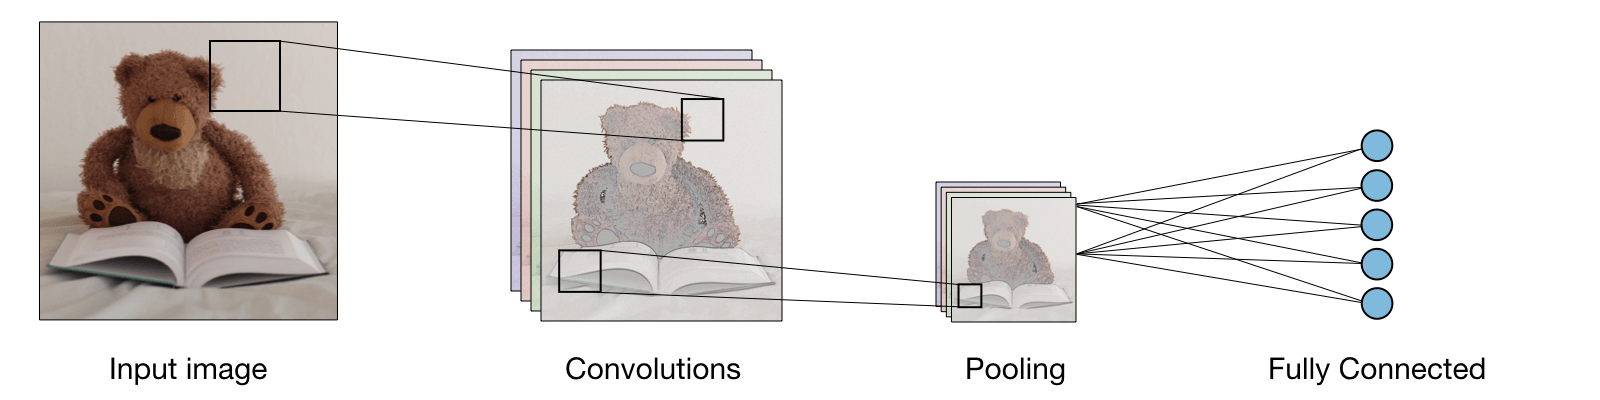
\includegraphics[width=0.65\textwidth]{bear}
        \end{figure}

        \begin{itemize}
            \item 
                Las capas convolucionales usa filtros que realizan operaciones de convolución mientras se
                escanea / pasa la \Quote{imagen} entrada, sus hiperparámetros incluyen el tamaño del filtro y el salto que se da,
                así como que es lo que pasa en las orillas de la imagen de entrada, la salida se llama mapa de características
                o mapa de activación.
            \item 
                Agrupación (pooling): Es una operación que busca la disminución de la resolución, 
                generalmente se aplica después de una capa de convolución; produce cierta invariancia espacial. 
                En particular, el max y mean pooling son tipos especiales de pooling donde 
                se toman el valor máximo y promedio, respectivamente.
            \item Lineares:
                Totalmente conectada: Funciona en una entrada aplanada donde cada entrada está conectada a todas
                las neuronas, para esto tenemos que \Quote{espagetificar} nuestra entrada, estas si están presentes,
                se encuentran hacia el final de la arquitectura y se pueden usar para optimizar objetivos
                como las probabilidades de una clase.
        \end{itemize}
        
        \section{Dropout}
            En pocas palabras, el dropout se refiere a ignorar unidades (es decir, neuronas) durante la fase de 
            entrenamiento de cierto conjunto de neuronas que se elige al azar. 
            
            Por \Quote{ignorar}, quiero decir que estas unidades no se consideran durante un pase particular 
            hacia adelante o hacia atrás.

            Más técnicamente, en cada etapa de entrenamiento, los nodos individuales se eliminan 
            de la red con probabilidad 1-p o se mantienen con probabilidad p, 
            de modo que queda una red reducida; Los bordes entrantes y salientes a un 
            nodo abandonado también se eliminan.

            \subsection{¿Por qué lo necesitamos?}
                ¿Por qué necesitamos literalmente apagar partes de una red neuronal?
                La respuesta a estas preguntas es para evitar el overfitting.

                Una capa totalmente conectada ocupa la mayoría de los parámetros y, por lo 
                tanto, las neuronas desarrollan una codependencia entre 
                ellas durante el entrenamiento, lo que frena el poder individual de cada neurona, 
                lo que lleva a un ajuste excesivo de los datos de entrenamiento.

                Para esto es que el dropout cae como anillo al dedo.

\part{Sistema de reconocimiento de objetos en imágenes}

    \chapter{El problema}

        El problema que elegí fue el predecir, dada una fotografía de una mano haciendo algo algún símbolo (letra)
        en lenguaje de signos, ser capaz de obtener la letra o símbolo descrito.
        
        \section{Importancia de resolverlo}

        La técnica del reconocimiento de objetos de manera automática en imágenes es muy usada en la industria,
        por ejemplo en los sistemas de navegación automonos de los autos siendo capaces de encontrar la linea en medio del
        camino o de encontrar y localizar a las personas dentro de una foto o poder leer los números de tu tarjeta con una foto de
        la misma.

        Este problema en particular creo que muy obvio la importancia: no todos nacemos o tenemos las mismas oportunidades
        por lo que buscar crear mediante la tecnología sistemas que nos permitan comunicarnos mejor es de vital importancia,
        sistemas como el que propongo aquí (ayudados de otro que nos permita encontrar manos dentro de una imagen) nos podrían
        ayudar a crear un sistema de apoyo para traducir de manera totalmente automática una conversación o un video en el
        que se use el lenguaje de signos.
        Permitiendo que sin mayor problema para el usuario se pueda crear un \Quote{transcript} que nos permita entender de manera
        escrita lo que una persona esta diciendo, o visto de otra manera podría ser el equivalente que tenemos de nuestros
        sistemas de dictado automática en el que presionamos un botón y empezamos a hablar, viendo como las palabras aparecen
        en tiempo real en la pantalla, podríamos usar este sistema que propongo como una pieza clave para poder crear un
        equivalente en el que alguien hable en lenguaje de señas y se pueda ver una transcripción en tiempo real del contenido,
        esto por ejemplo también seria muy útil para conferencias y videoconferencias / reuniones online.

        Es decir, un buen algoritmo que resuelva este problema podría ayudar de manera pragmática a las personas
        sordas y con dificultades auditivas a comunicarse mejor utilizando aplicaciones de visión por computadora.

        El Instituto Nacional de Sordera y otros Trastornos de las Comunicaciones (NIDCD)
        indica que el lenguaje de señas americano de 200 años es un lenguaje completo y complejo
        (del cual los gestos con letras son solo una parte), pero es el idioma principal para
        muchos norteamericanos sordos.

        El ASL es el idioma minoritario líder en los Estados Unidos después de los \Quote{cuatro grandes}: español, italiano,
        alemán y francés. Se podría implementar la visión por computadora en una computadora de tablero económica
        como Raspberry Pi con OpenCV, y algunas Text-to-Speech para permitir aplicaciones
        de traducción mejoradas y automatizadas.


        \begin{figure}[ht!]
            \centering
            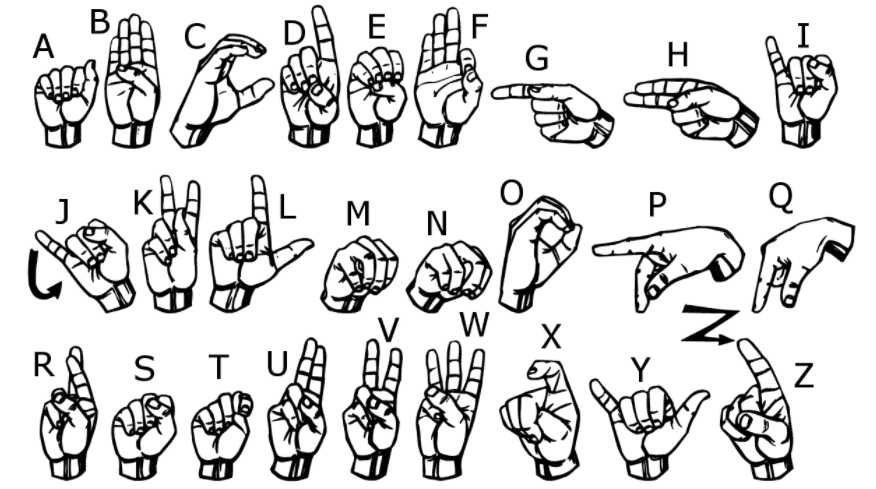
\includegraphics[width=0.65\textwidth]{images}
        \end{figure}

    \chapter{El dataset / Business Understanding}

        En mi caso el dataset que balanceaba más unos datos limpios con una gran cantidad de información fue uno bastante famoso:
        MNIST Sign Language:
        
        El conjunto de datos de imagen original MNIST, ya saben el que todos conocemos de los dígitos escritos a mano es un
        punto de referencia bastante popular para los métodos de aprendizaje automático,
        pero los investigadores han renovado sus esfuerzos para actualizarlo y desarrollar reemplazos
        directos que son más desafiantes para la visión por computadora y originales para aplicaciones del mundo real.
        
        El MNIST que se presenta aquí sigue el mismo formato CSV con etiquetas y valores de píxeles en filas individuales.
        La base de datos de gestos con las manos en lenguaje de señas americano representa un
        problema de varias clases con 24 clases de letras (excluyendo J y Z que requieren movimiento).
        Por eso mismo solo vamos a usar 25 clases (podríamos hacer 24, pero dado que la clase que falta es la 9 pensé más coherente
        dejarlas en 25).
        
        El formato del conjunto de datos está diseñado para coincidir estrechamente con el clásico MNIST.
        Cada caso de entrenamiento y prueba representa una etiqueta (0-25) como un mapa uno a uno para cada
        letra alfabética A-Z (y no hay casos para 9 = J o 25 = Z debido a movimientos gestuales).
        Los datos de entrenamiento (27,455 casos) y los datos de prueba (7172 casos) son aproximadamente la mitad
        del tamaño del MNIST estándar, pero por lo demás son similares con una fila de encabezado de etiqueta,
        pixel1, pixel2 ... .pixel784 que representa una sola imagen de 28x28 píxeles con valores de escala de
        grises entre 0-255.
        
        Los datos originales de la imagen del gesto de la mano representaban a múltiples usuarios que
        repetían el gesto en diferentes fondos. Los datos del lenguaje de señas MNIST provienen de una
        gran extensión del pequeño número (1704) de las imágenes en color incluidas como no recortadas alrededor de
        la región de interés de la mano. Para crear nuevos datos, se usó una tubería de imagen basada en ImageMagick e
        incluyó el recorte a solo manos, escala de grises, cambio de tamaño y luego crear al menos más de 50 variaciones
        para aumentar la cantidad.
        
        La estrategia de modificación y expansión fue filtros ('Mitchell', 'Robidoux', 'Catrom', 'Spline', 'Hermite'),
        junto con un 5\% de pixelación aleatoria, +/- 15\% de brillo / contraste, y finalmente una rotación de 3 grados.
        Debido al pequeño tamaño de las imágenes, estas modificaciones alteran efectivamente la resolución y
        la separación de clases de formas interesantes y controlables.
        
        Este conjunto de datos se inspiró en el Fashion-MNIST 2 y la línea de aprendizaje automático para gestos de Sreehari 4.
        
        En mi caso lo descarge de Kaggle y lo pueden encontrar en el siguiente link:
        \url{https://www.kaggle.com/datamunge/sign-language-mnist}
        
        El problema es que por la velocidad de mi computadora el entrenamiento lo hice en colab y dado que con mi internet actualmente
        me hubiera tomado un par de horas descargar y subir a drive el dataset preferí subirlo a github y linkearlo de manera
        directa en Google Colab.

        \begin{figure}[ht!]
            \centering
            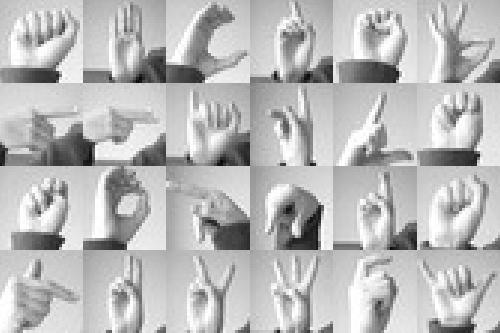
\includegraphics[width=0.65\textwidth]{bnw}
        \end{figure}

        \clearpage

        Podemos explorar el dataset con el siguiente código que hice:
        \begin{figure}[ht!]
            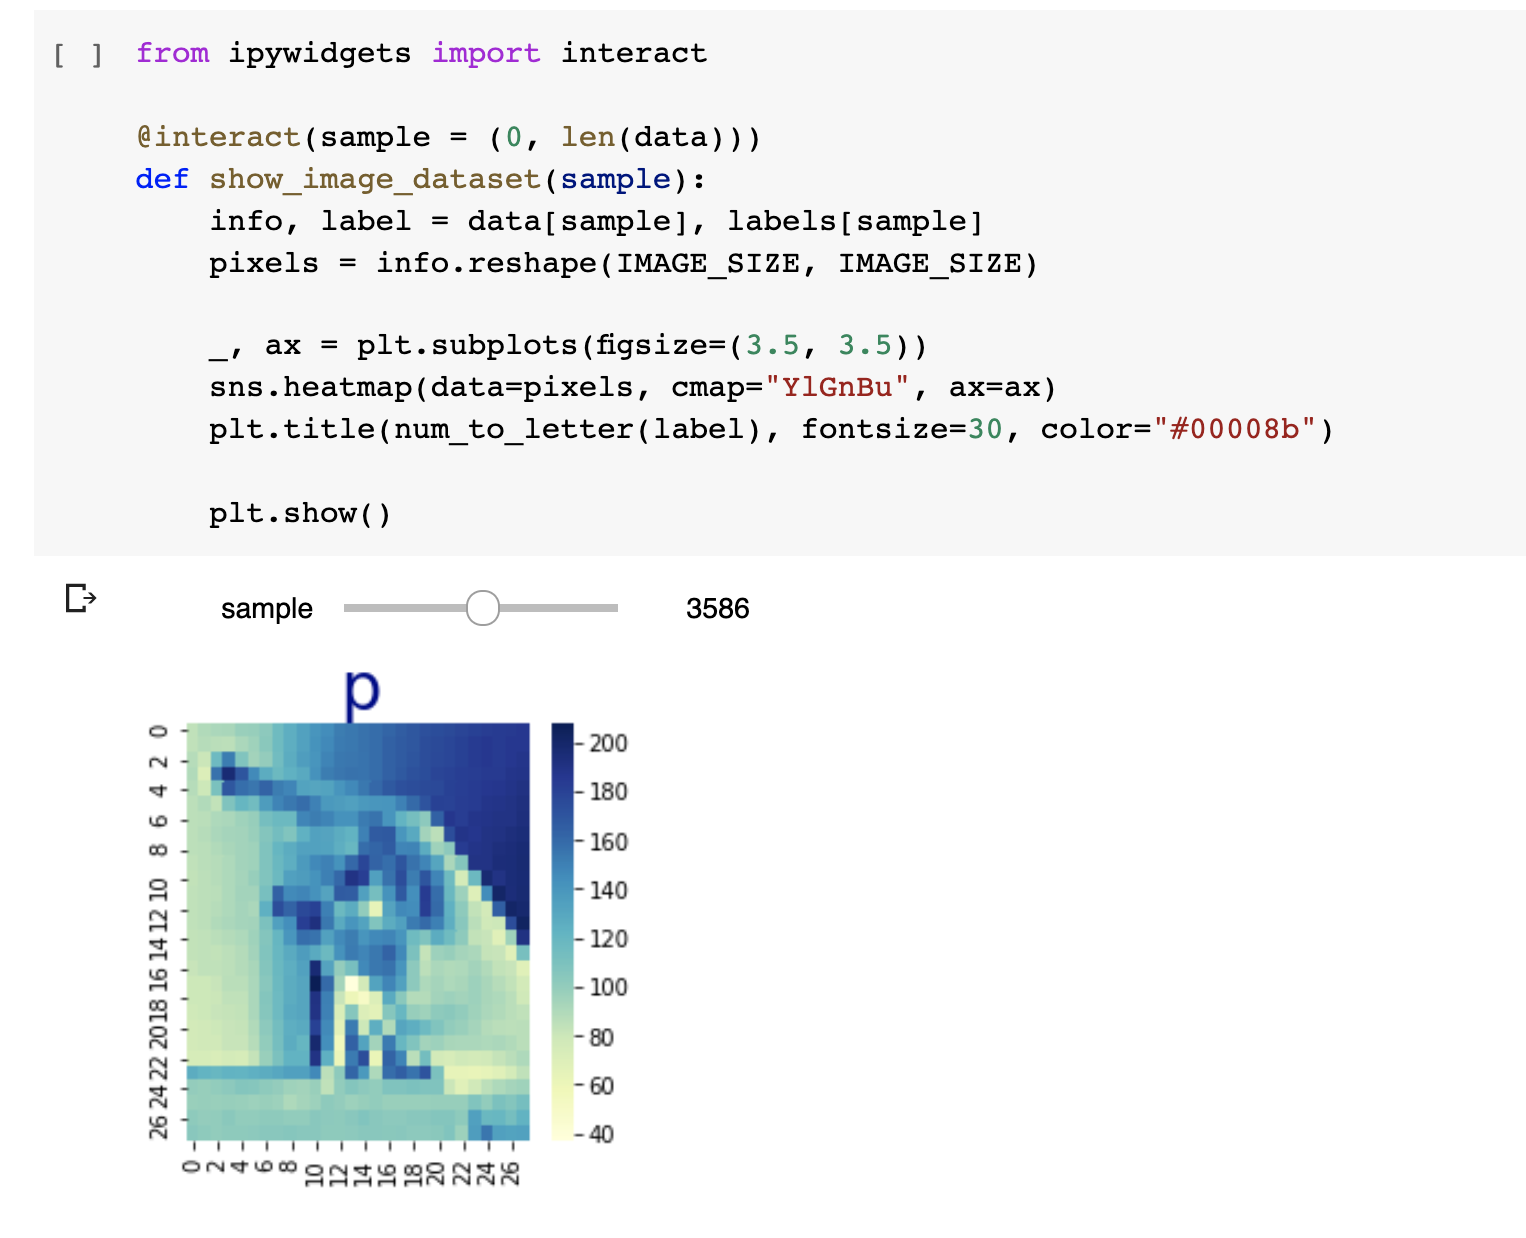
\includegraphics[width=0.45\textwidth]{see}
        \end{figure}

        Esto lo hago con ayuda de seaborn y uso un map de color azul, para no ver el clásico blanco y negro, los invito
        a probarlo en mi código.
        
        Ademas podemos de manera casi inmediata ver como están distribuidos las clases dentro del entrenamiento para ver
        si es que tenemos un dataset balanceado o no, a lo que yo concluyo que si bien no esta perfectamente balanceado
        creo que las variaciones son lo suficientemente pequeñas para no preocuparnos mucho de eso.
        
        Podemos explorar el dataset con el siguiente código que hice:
        \begin{figure}[ht!]
            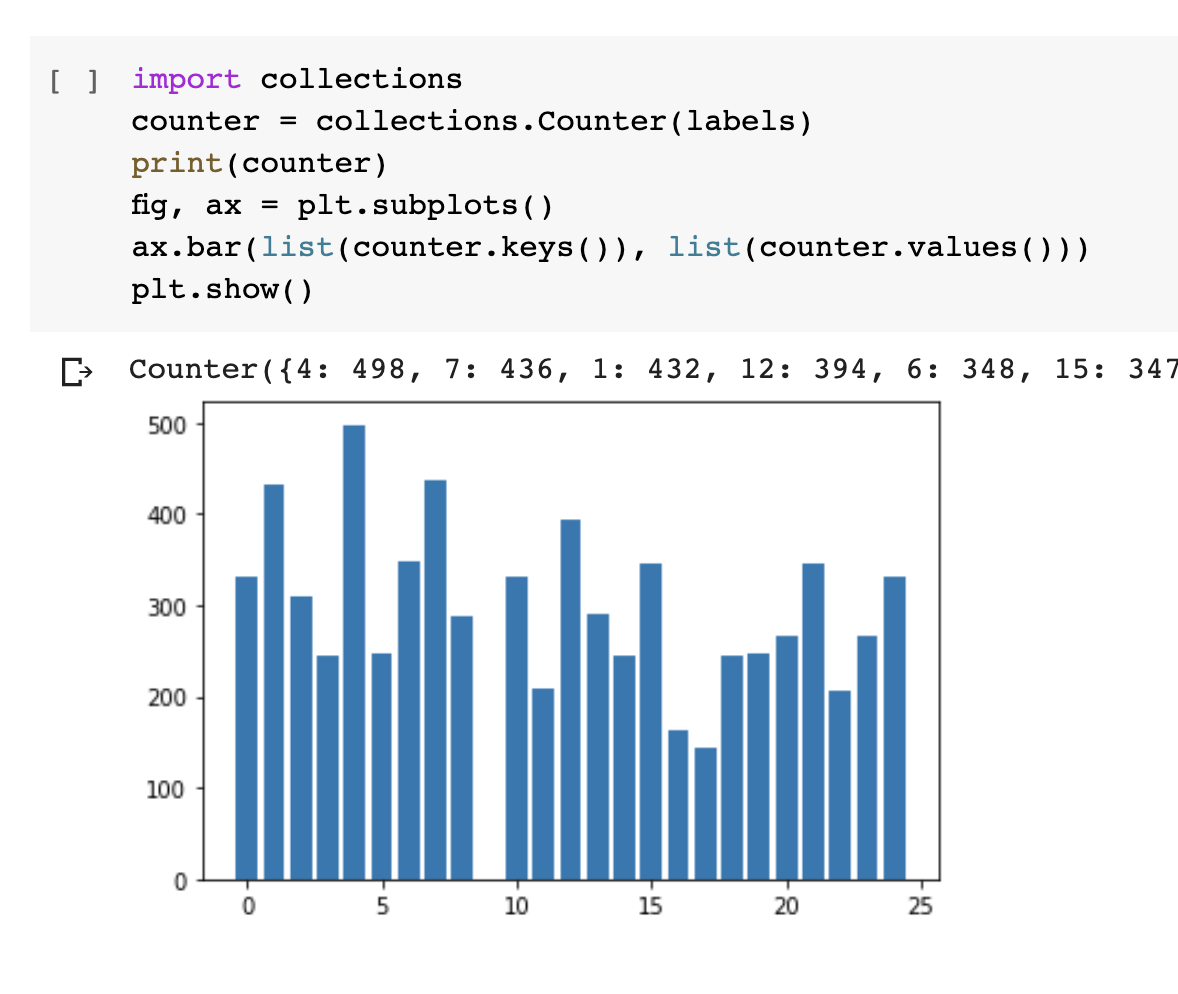
\includegraphics[width=0.45\textwidth]{dist}
        \end{figure}


    \chapter{La propuesta}
        Mi hipótesis sería que usando este dataset y
        mediante aprendizaje supervisado (redes neuronales, en especial convolucionales y usando algo de dropout) se podría
        crear un sistema que fuera capaz de clasificar con un gran alto nivel de exactitud (accuracy) (alrededor de un 85\%).
        
        Las redes neuronales convolucionales fueron elegidas por los puntos anteriormente dichos:
        sobre todo por la gran capacidad que tiene a la hora de clasificar (con la ayuda de capaz lineales) objetos dentro
        de una imagen, ademas que gracias al uso de Colab puedo tener acceso a una buena GPU con la que podemos hacer
        muchos más experimentos e iterar bastante rápido, ademas decidí usar dropout después de las redes convolucionales para
        eliminar algo de la dependencia de las neuronas y evitar con ello el overfitting.
        
        La principal desventaja de esta propuesta, es decir de usar redes neuronales convolucionales es que
        encontrar el valor ideales para los hiper parámetros es algo que no trivial,
        ademas de necesitar una gran dataset para tener resultados decentes y finalmente que es al final de cuentas una caja negra
        que cuesta bastante interpretar, por lo que incluso si se logra el objetivo sera bastante difícil entender que es lo que
        está haciendo nuestra red neuronal y porque esta eligiendo esta clase en vez de otra.
        
        Ademas de que el cálculo foward incluso ya entrenada no es tan rápido por lo cual toma un equipo con unas buenas características
        para poder hacer una detección en tiempo real.

        \clearpage
        Algo también importante es hablar sobre el espacio de hipótesis de esta idea, este
        depende del número de variables y los valores que puedan tomar esas variables.
        En nuestro caso veamos todos los parametros o pesos de la propuesta final que codifique para que nos demos una idea de la cantidad
        de parametros que hay que hacerles \Quote{fine tunning}:

        \begin{figure}[h!]
            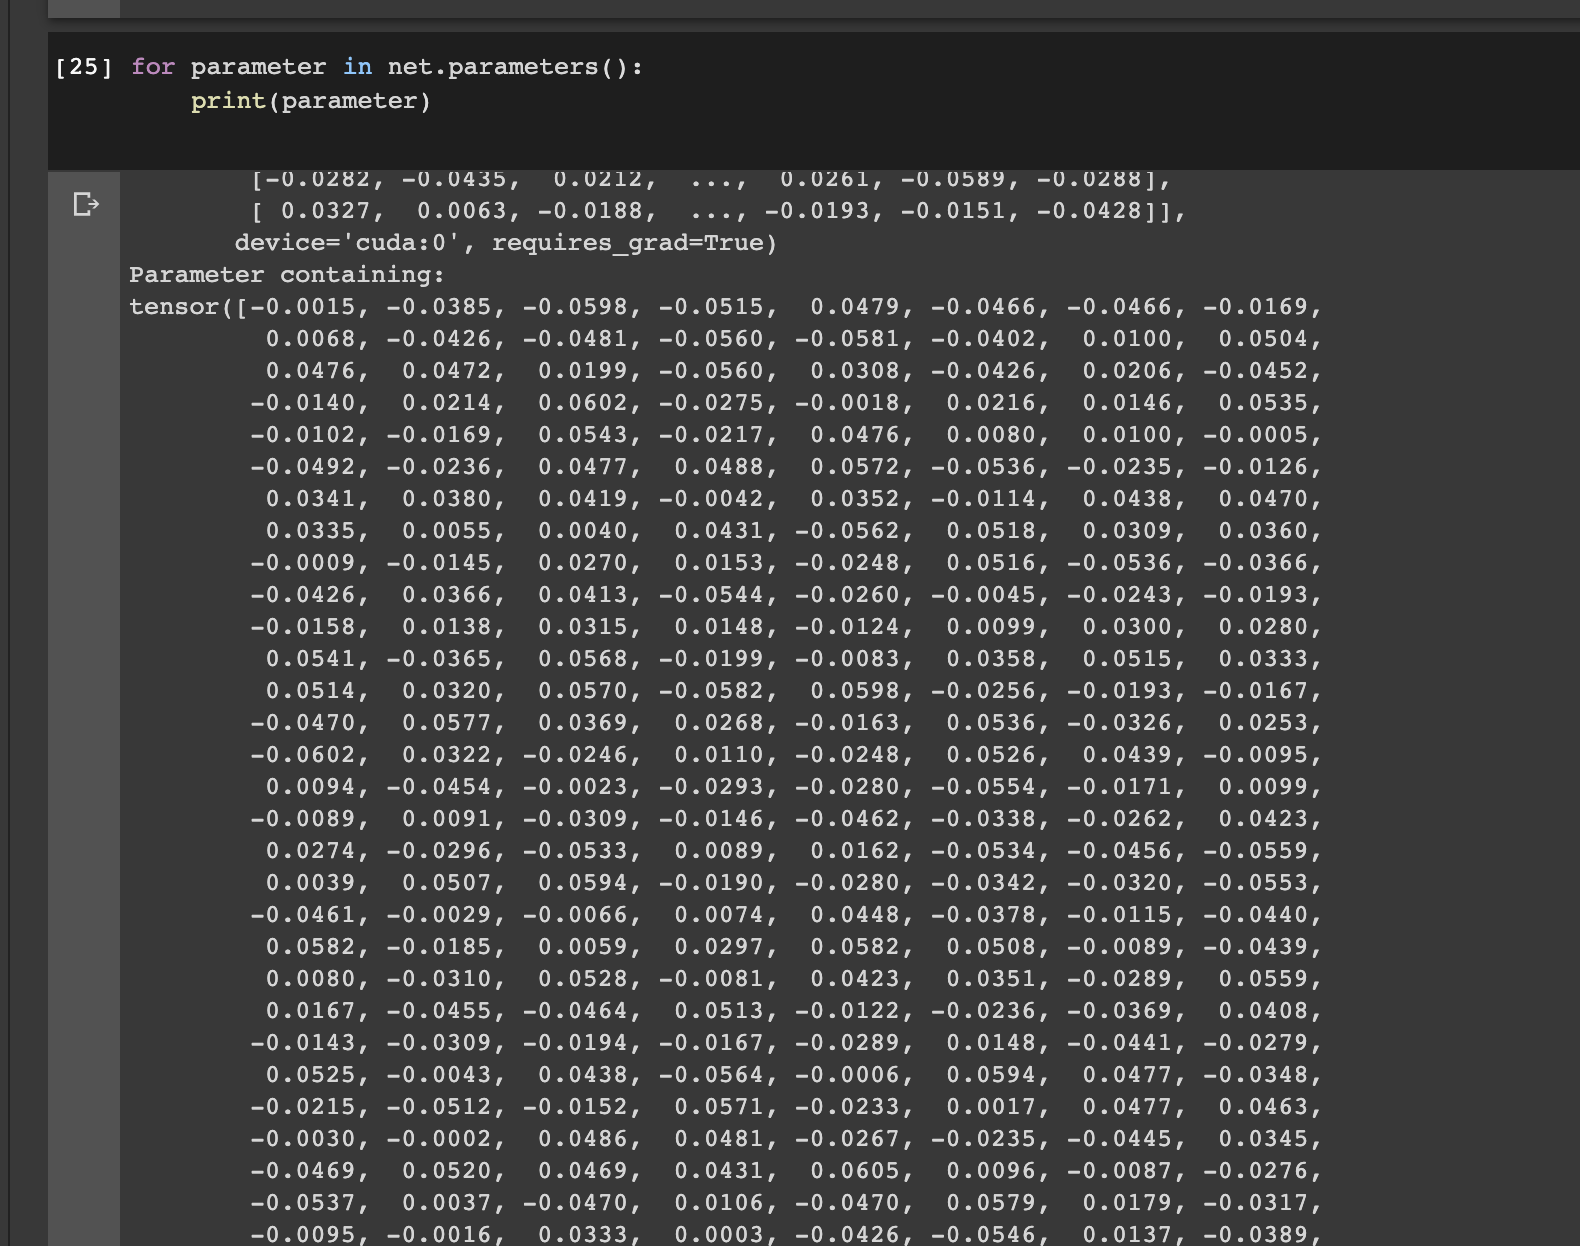
\includegraphics[width=0.4\textwidth]{a}

            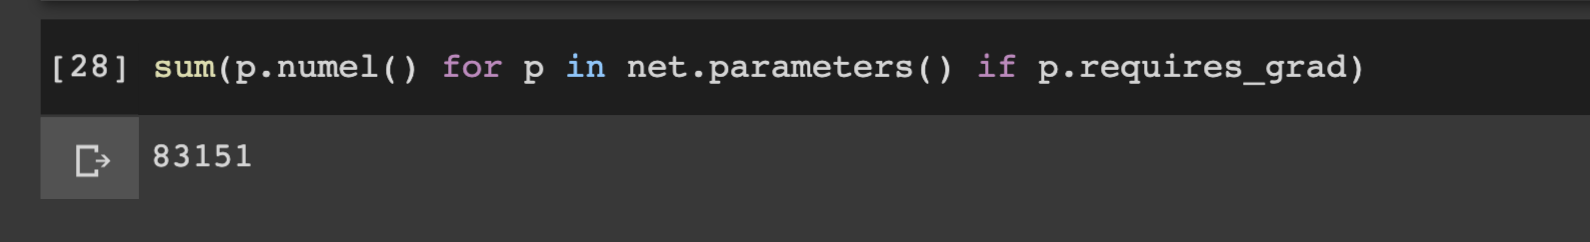
\includegraphics[width=0.8\textwidth]{b}
        \end{figure}

        Como podemos ver, no son pocos, de hecho llegamos cerca de los 100, 000 parametros que vamos a modificar, esto nos da
        una escala de cuan difícil de resolver es tu problema.

    \chapter{La implementación}

        \section{Preparación de los datos}

        Lo primero que tuvimos que hacer fue preparar los datos, es decir descargarlos, y poder separar nuestra información
        entre training, test y validation, vimos el tamaño de cada una:

        \begin{figure}[h!]
            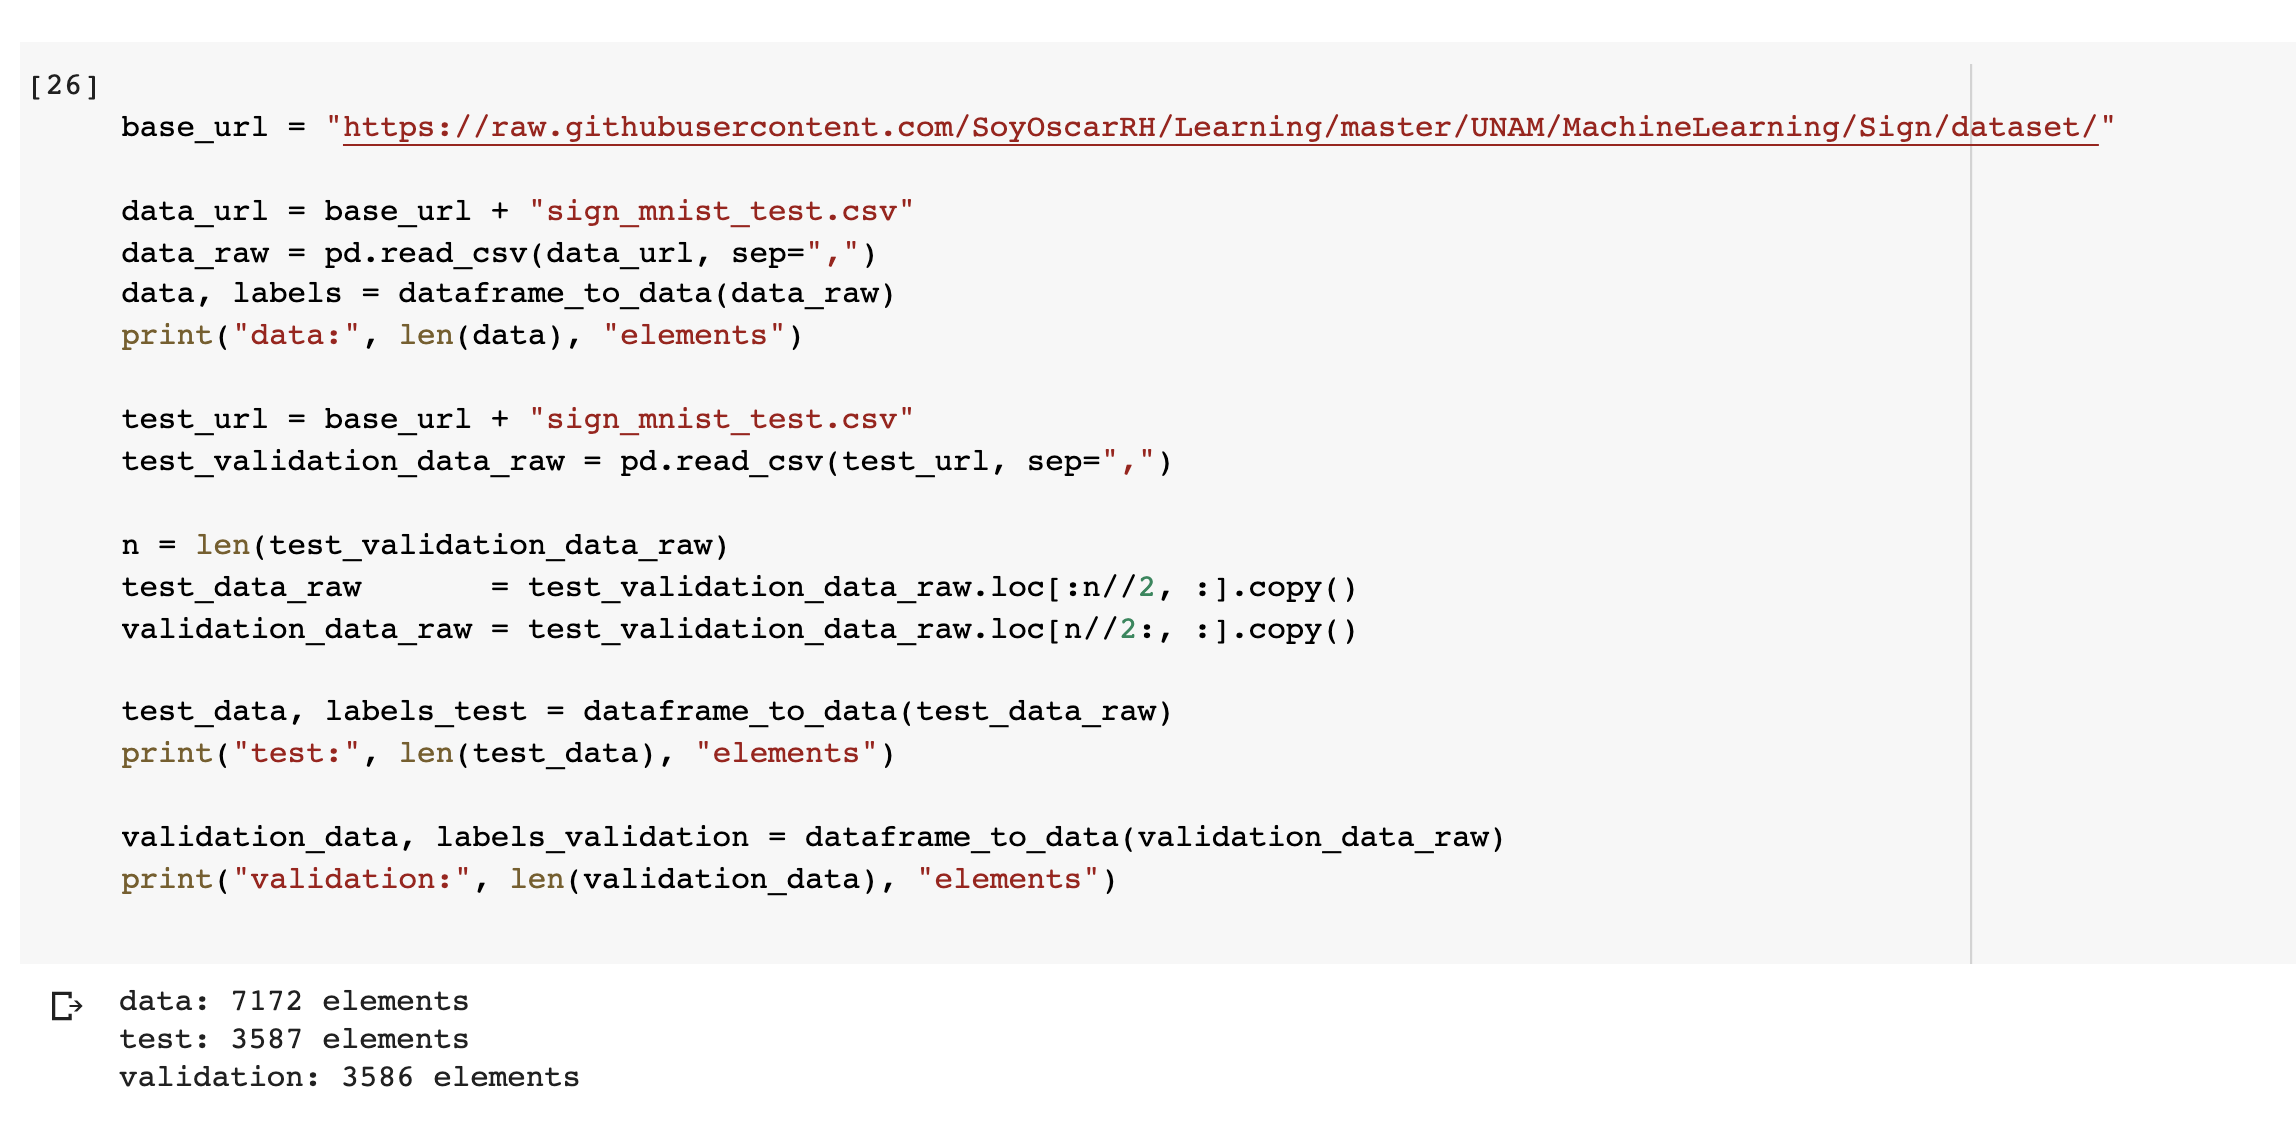
\includegraphics[width=0.5\textwidth]{1}
            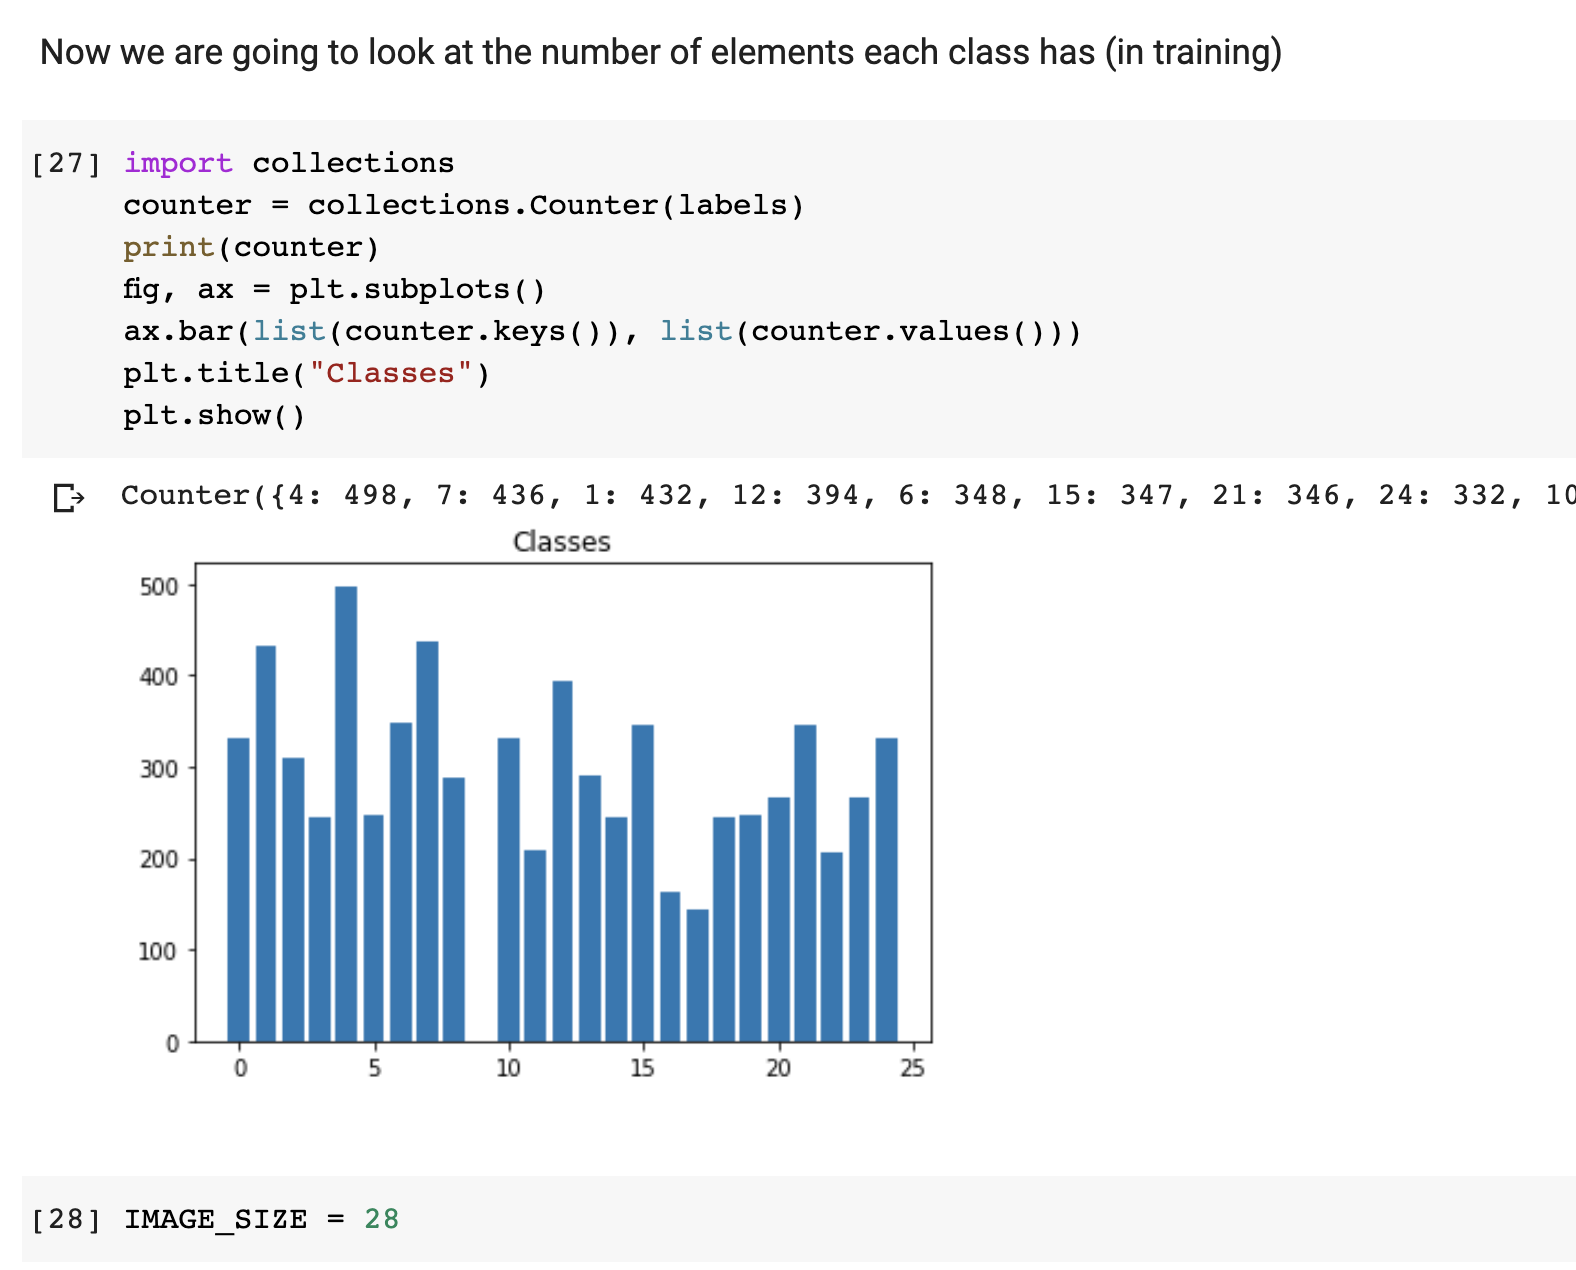
\includegraphics[width=0.5\textwidth]{2}
        \end{figure}

        \clearpage

        Con esto listo como dije antes podemos ver que tan balanceadas estaban las clases y cree un pequeño widget
        que te permite explorar fácilmente el dataset.

        \begin{figure}[h!]
            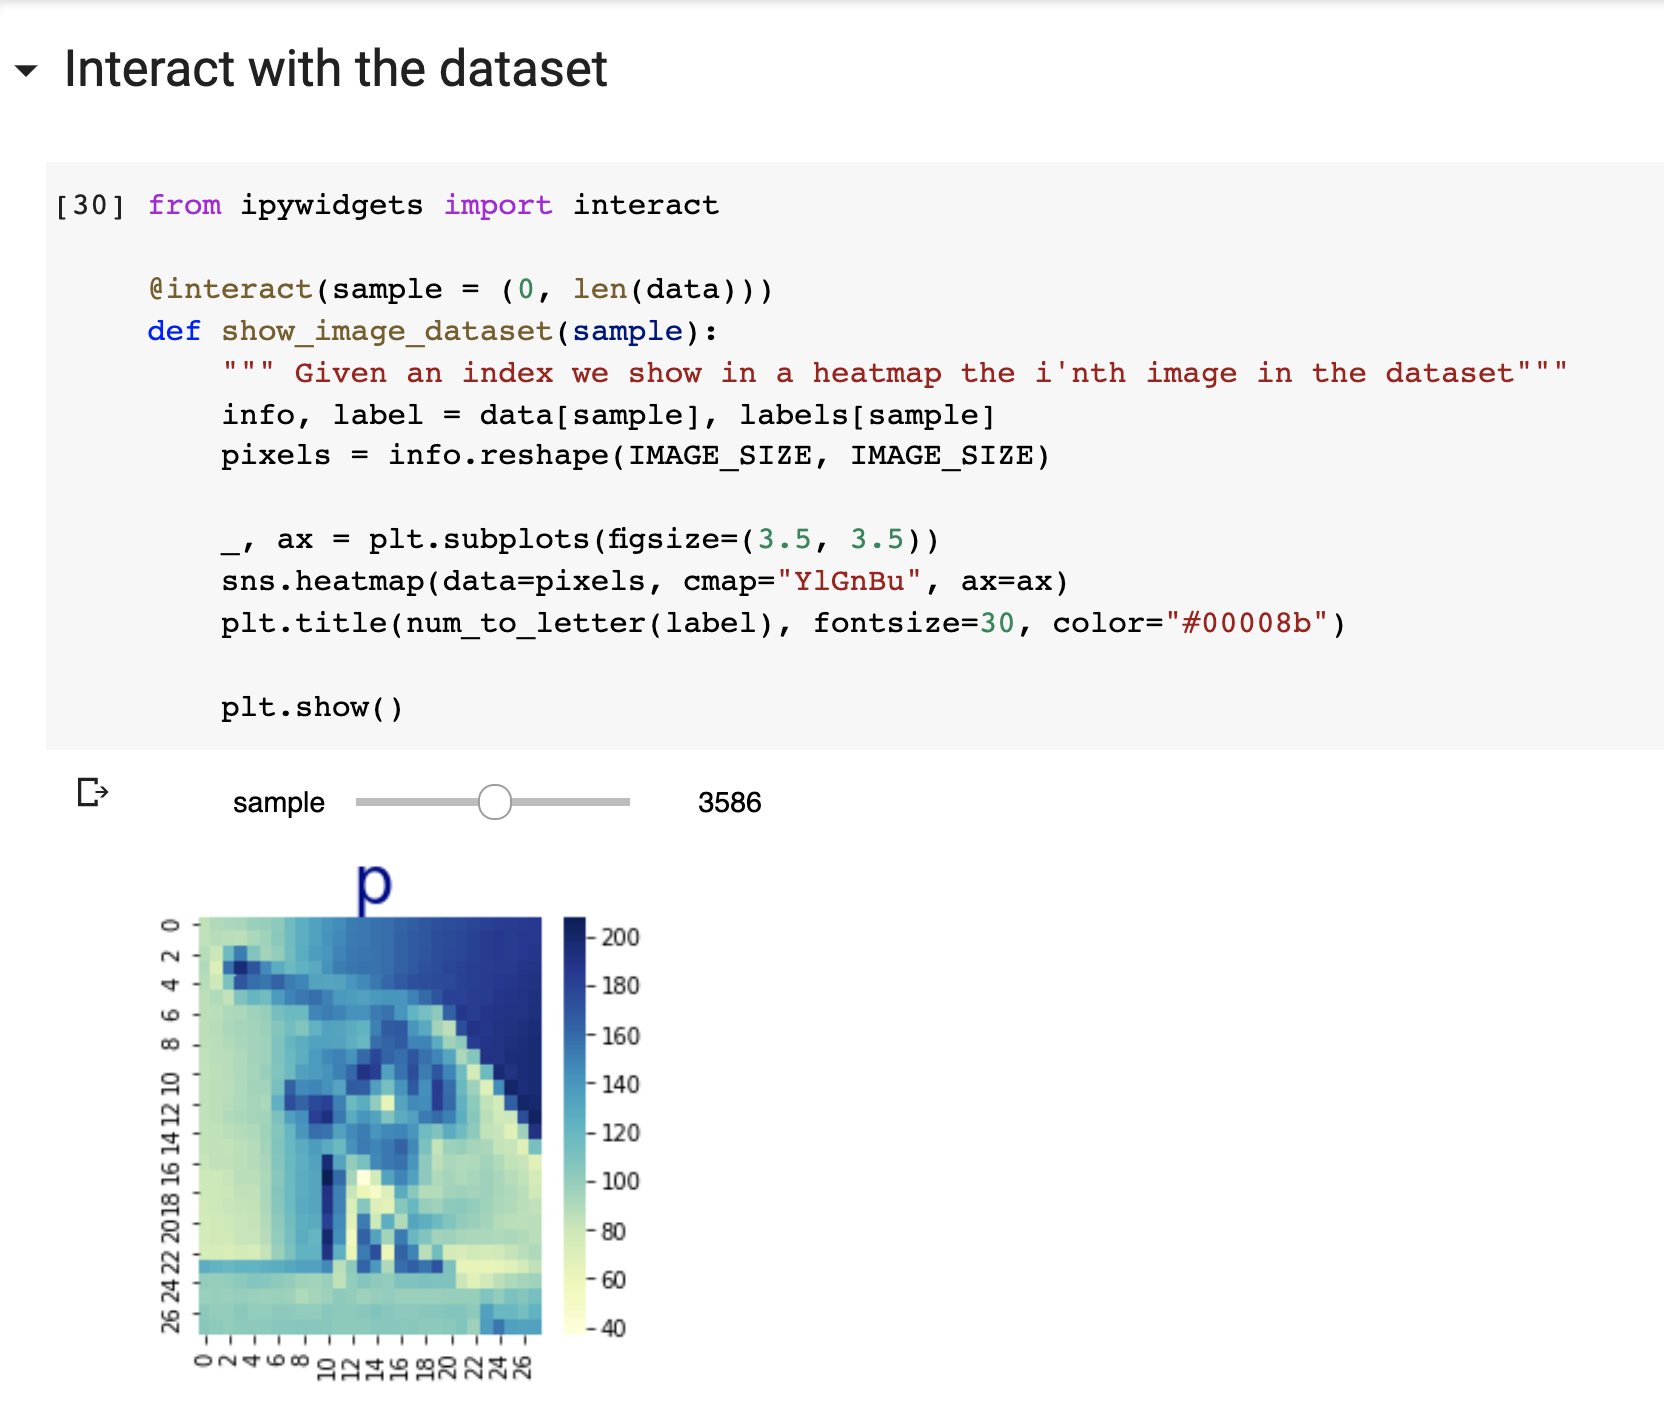
\includegraphics[width=0.65\textwidth]{3}
        \end{figure}

        \clearpage
        \section{Creación del clasificador}

        Esto fue mucho más sencillo de que esperaba, nuestro primer paso semi previo fue el de tomar nuestros datos y volverlos
        tensores para que pytorch los pueda entender.

        \begin{figure}[h!]
            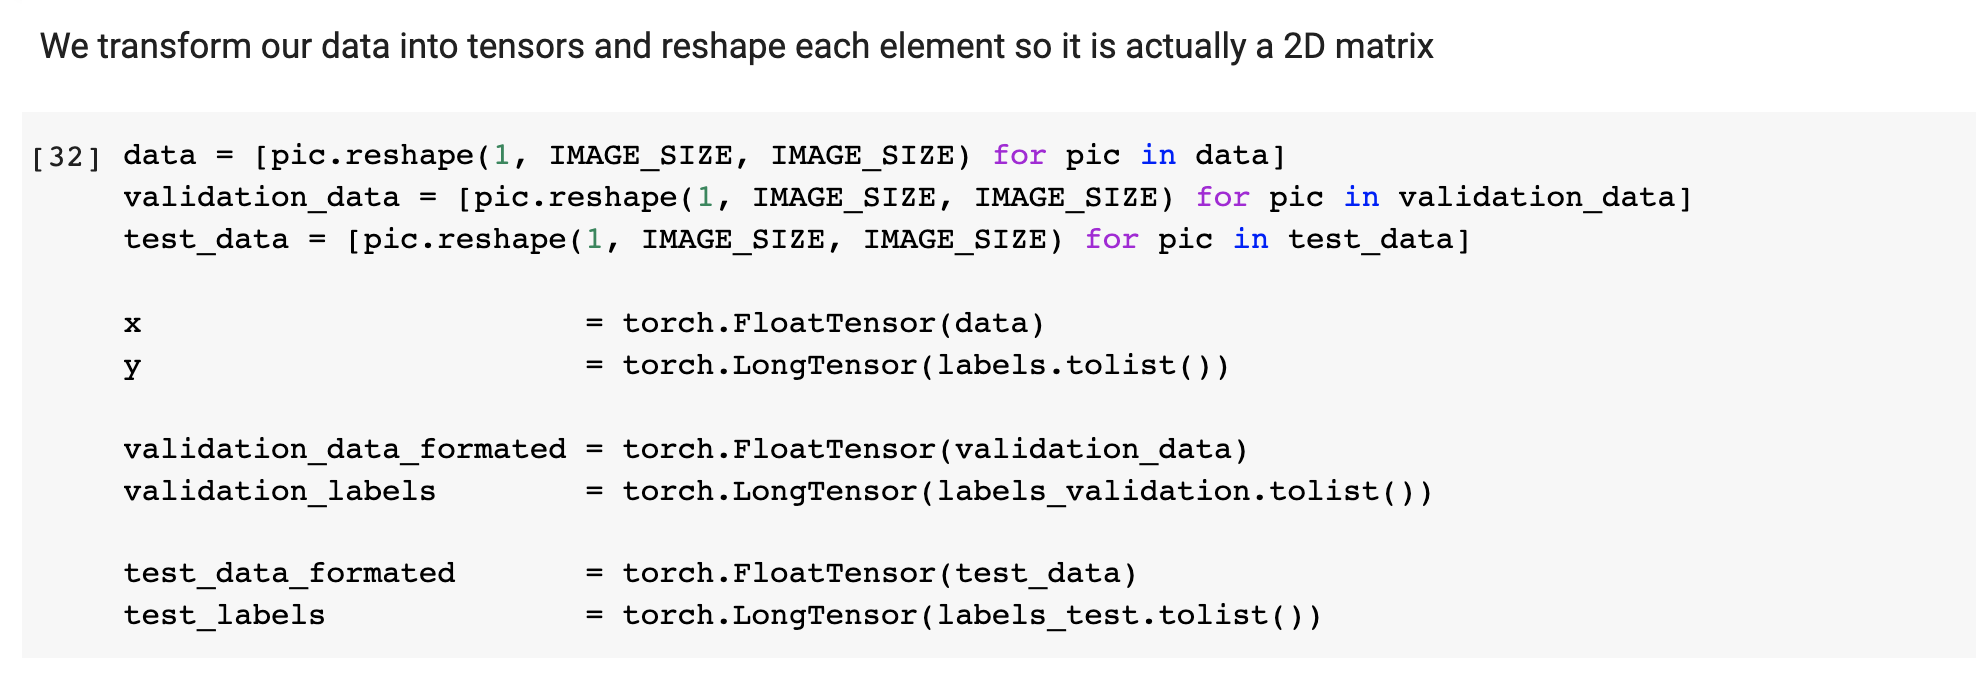
\includegraphics[width=0.65\textwidth]{4}
        \end{figure}

        Después declaramos nuestra red neuronal, para ser exactos usando pytorch y para trabajar con esta librería tenemos
        que implementar dos métodos, un constructor que nos declarara que elementos tiene nuestra arquitectura y una función
        llamada foward que nos permite expresar el flujo de nuestros datos.

        Así que vamos a explicar mas a detalle:
        Como entrada a nuestros sistema no tendremos una simple imagen en 2d, es decir una matriz, sino que como trabajamos como
        batch tendremos un arreglo de matrices, nuestro primer paso sera pasar por unas capas convolucionales,
        como es en blanco y negro usamos solo un canal de entrada y usando un kernel de 3x3 tendremos 10 filtros de salida,
        estos serán reducidos usando max pooling de 2x2, con esto nuestra información entra a la siguiente capa, dentro de ella
        repetiremos el mismo proceso ahora incrementando en 10 nuestros filtros de salida.

        De tal manera que al final hemos pasado por 3 capas convolucionales y ahora usaremos dropout para mejorar
        el entrenamiento y evitar el overfitting con una probabilidad bastante alta de un 0.4.

        Finalmente hay que tomar las salidas y espagetificarlas, en este caso deje el cálculo tal cual para que sea más obvio
        porque esa capa conexa requiere esas conexiones, finalmente esta capa tiene 256 neuronas ocultas que son tomadas por
        la siguiente capa teniendo las 25 clases de salida.

        Entre las capaz lineales usamos una simple relu y nuestro trabajo aquí esta listo.
        \begin{figure}[h!]
            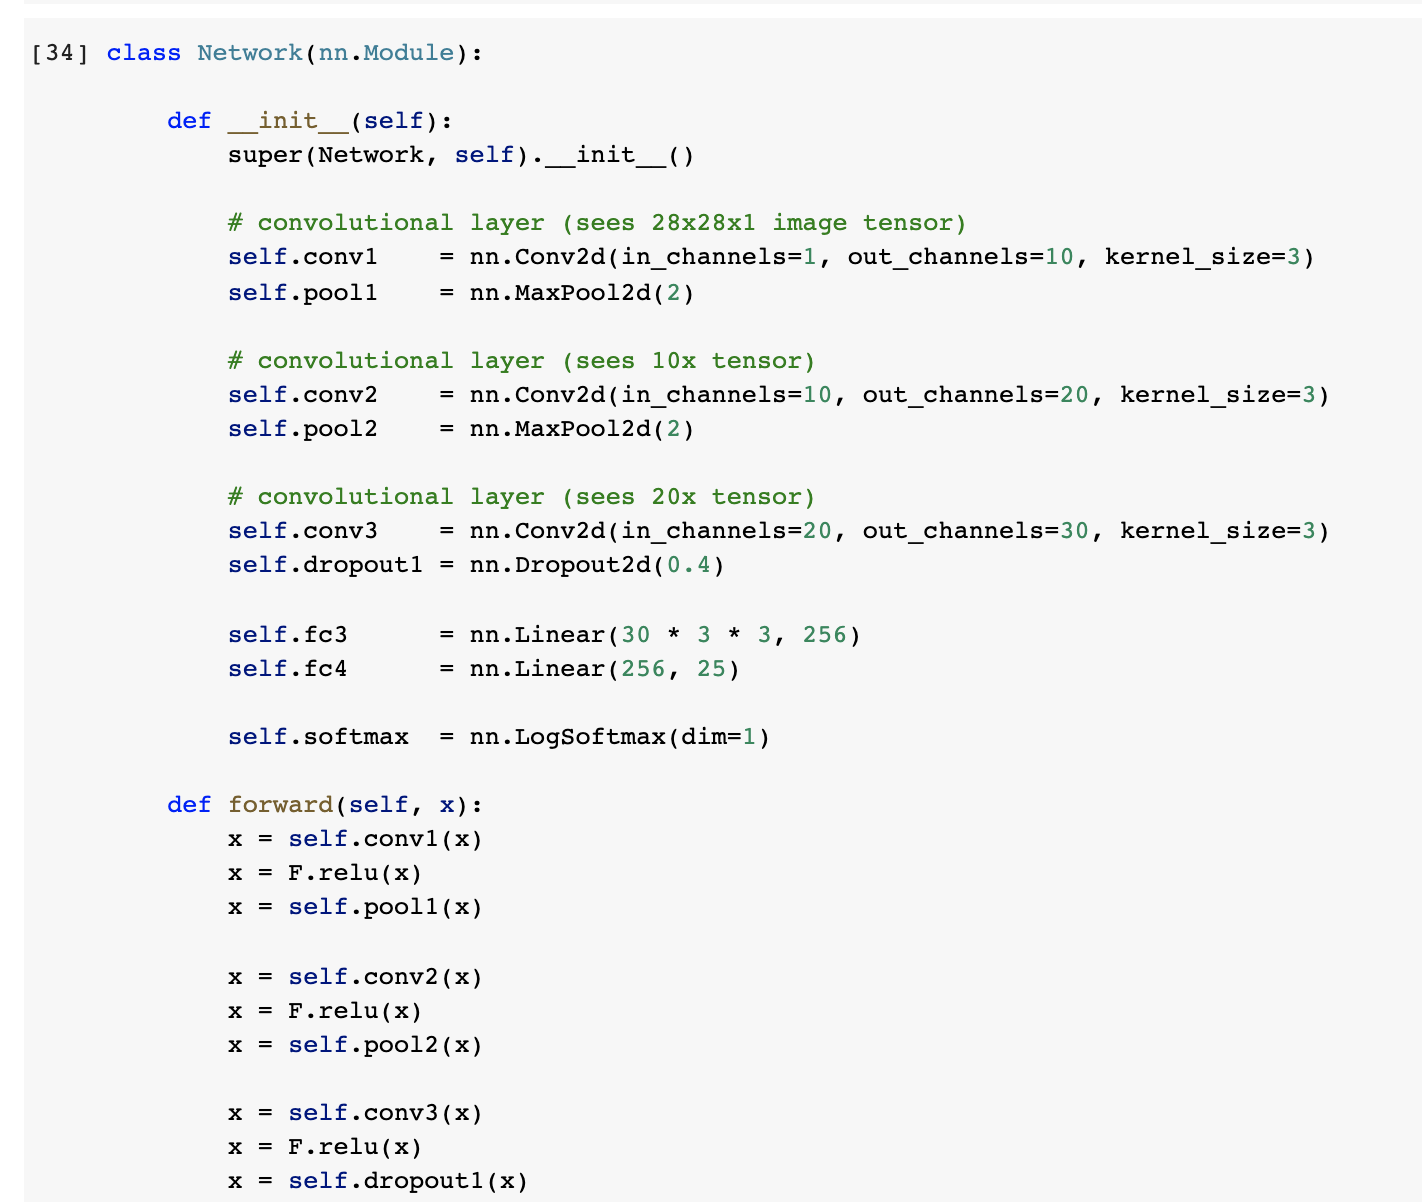
\includegraphics[width=0.65\textwidth]{6}
        \end{figure}

        \clearpage
        Tambien les damos valor a unos cuantos hiperparametros:
        \begin{figure}[h!]
            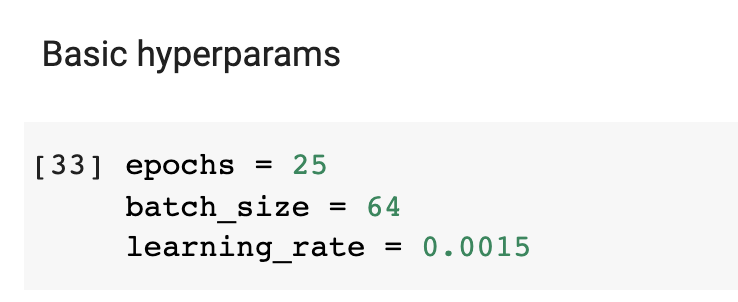
\includegraphics[width=0.35\textwidth]{5}
        \end{figure}

        Finalmente y para hacer reproducible a nuestro modelo usaremos una semilla fija para la generación de números aleatorios
        y ademas usaremos cuda de ser posible, con esto podemos ver de manera más compacta todo lo importante de nuestra red:
        \begin{figure}[h!]
            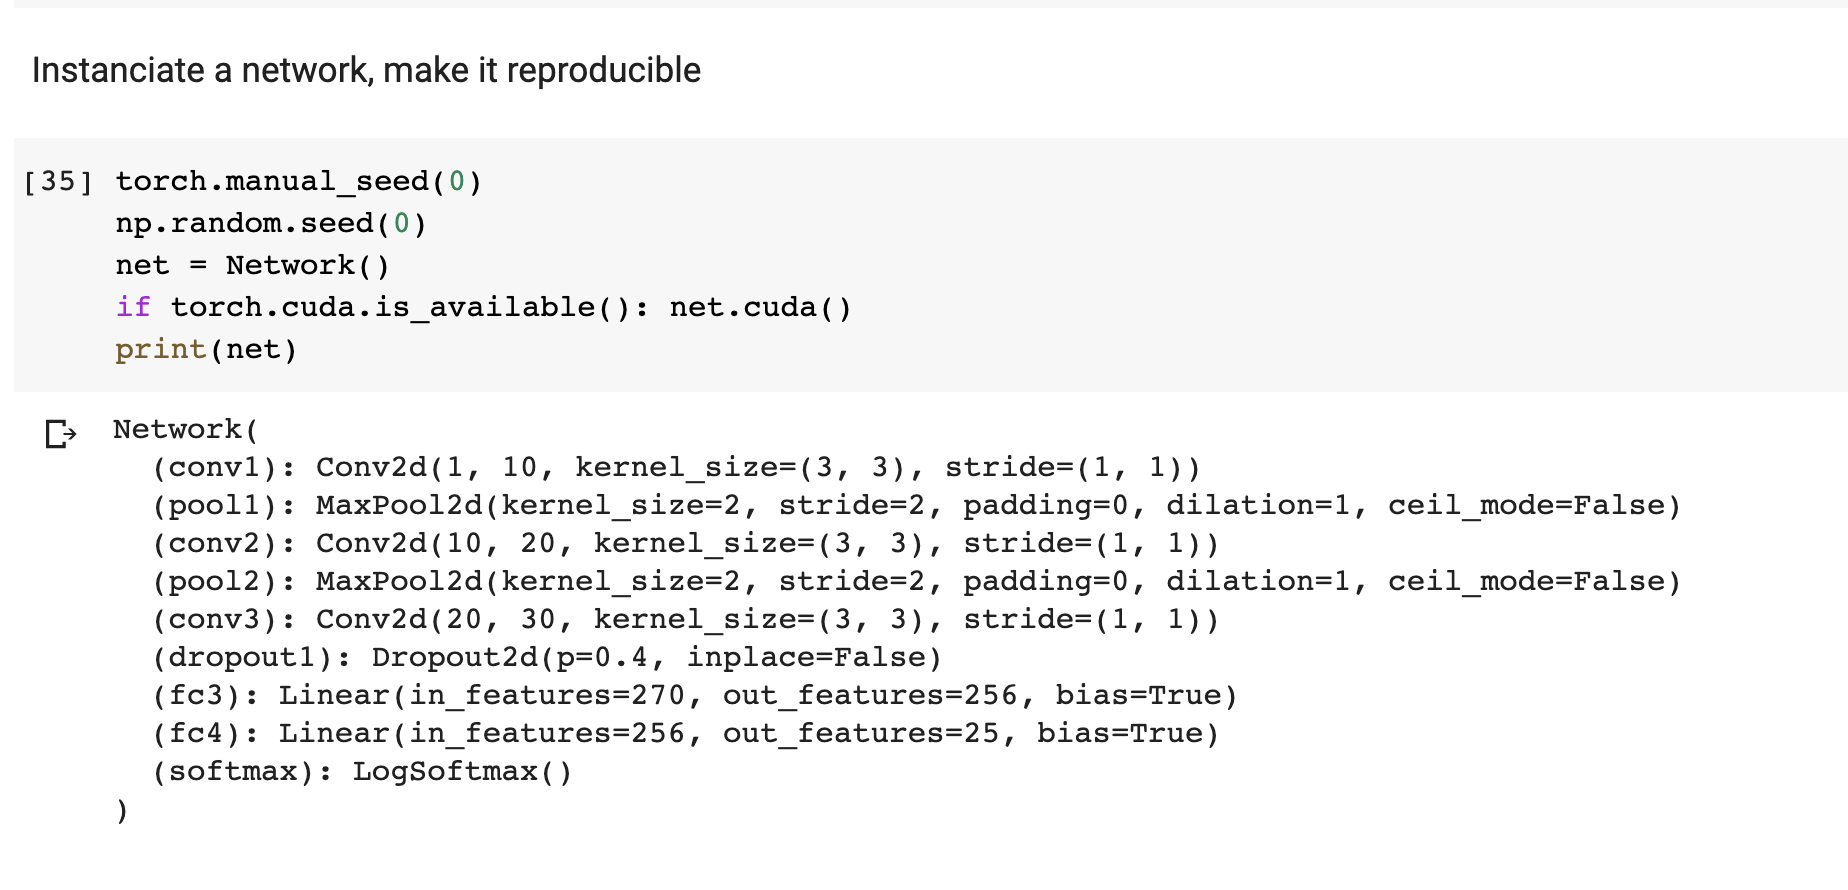
\includegraphics[width=0.65\textwidth]{7}
        \end{figure}

        Finalmente y no menos importante usamos tanto una función clásica de optimización como es SGD o stocastic gradient descent
        con un momentum del 0.7 y como estamos haciendo clasificación con más de dos clases el función de perdida estándar es
        entropía cruzada.

        \begin{figure}[h!]
            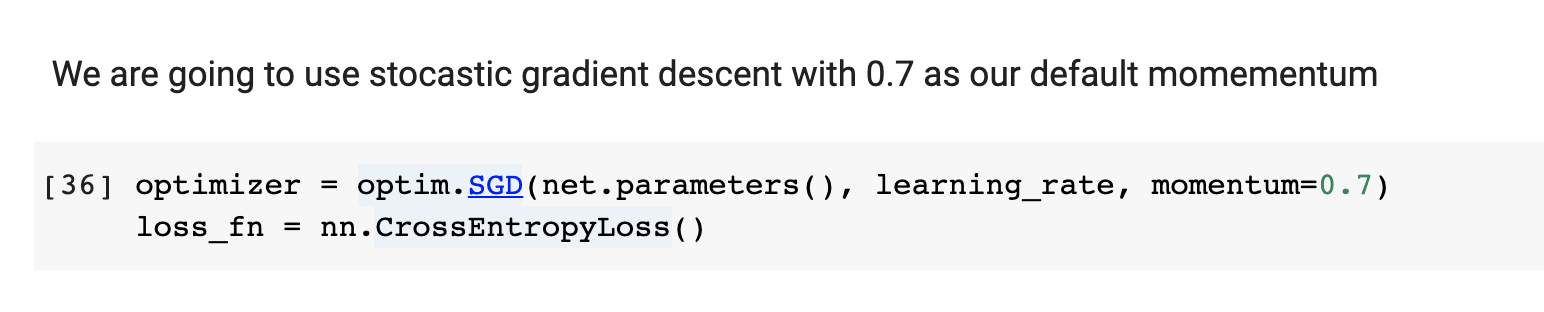
\includegraphics[width=0.45\textwidth]{8}
        \end{figure}

        \clearpage

        \section{Training Loop}

        Ahora con la arquitectura ya definida vamos a hacer el training loop, donde iremos alimentando a nuestra red neuronal con
        batches de datos y viendo como es que va la perdida, en este caso use dos perdidas, tanto la de entrenamiento, que espero
        que siempre baje como la de validación que empezara a subir si es que tenemos un modelo que hace overfitting, para evitarlo
        cada que alcancemos un mínimo en nuestro error de validación vamos a guardar los pesos del modelo, de tan manera que tras
        las epochs que pusimos nos podamos quedar con el mejor modelo, no solo el ultimo.

        \begin{figure}[h!]
            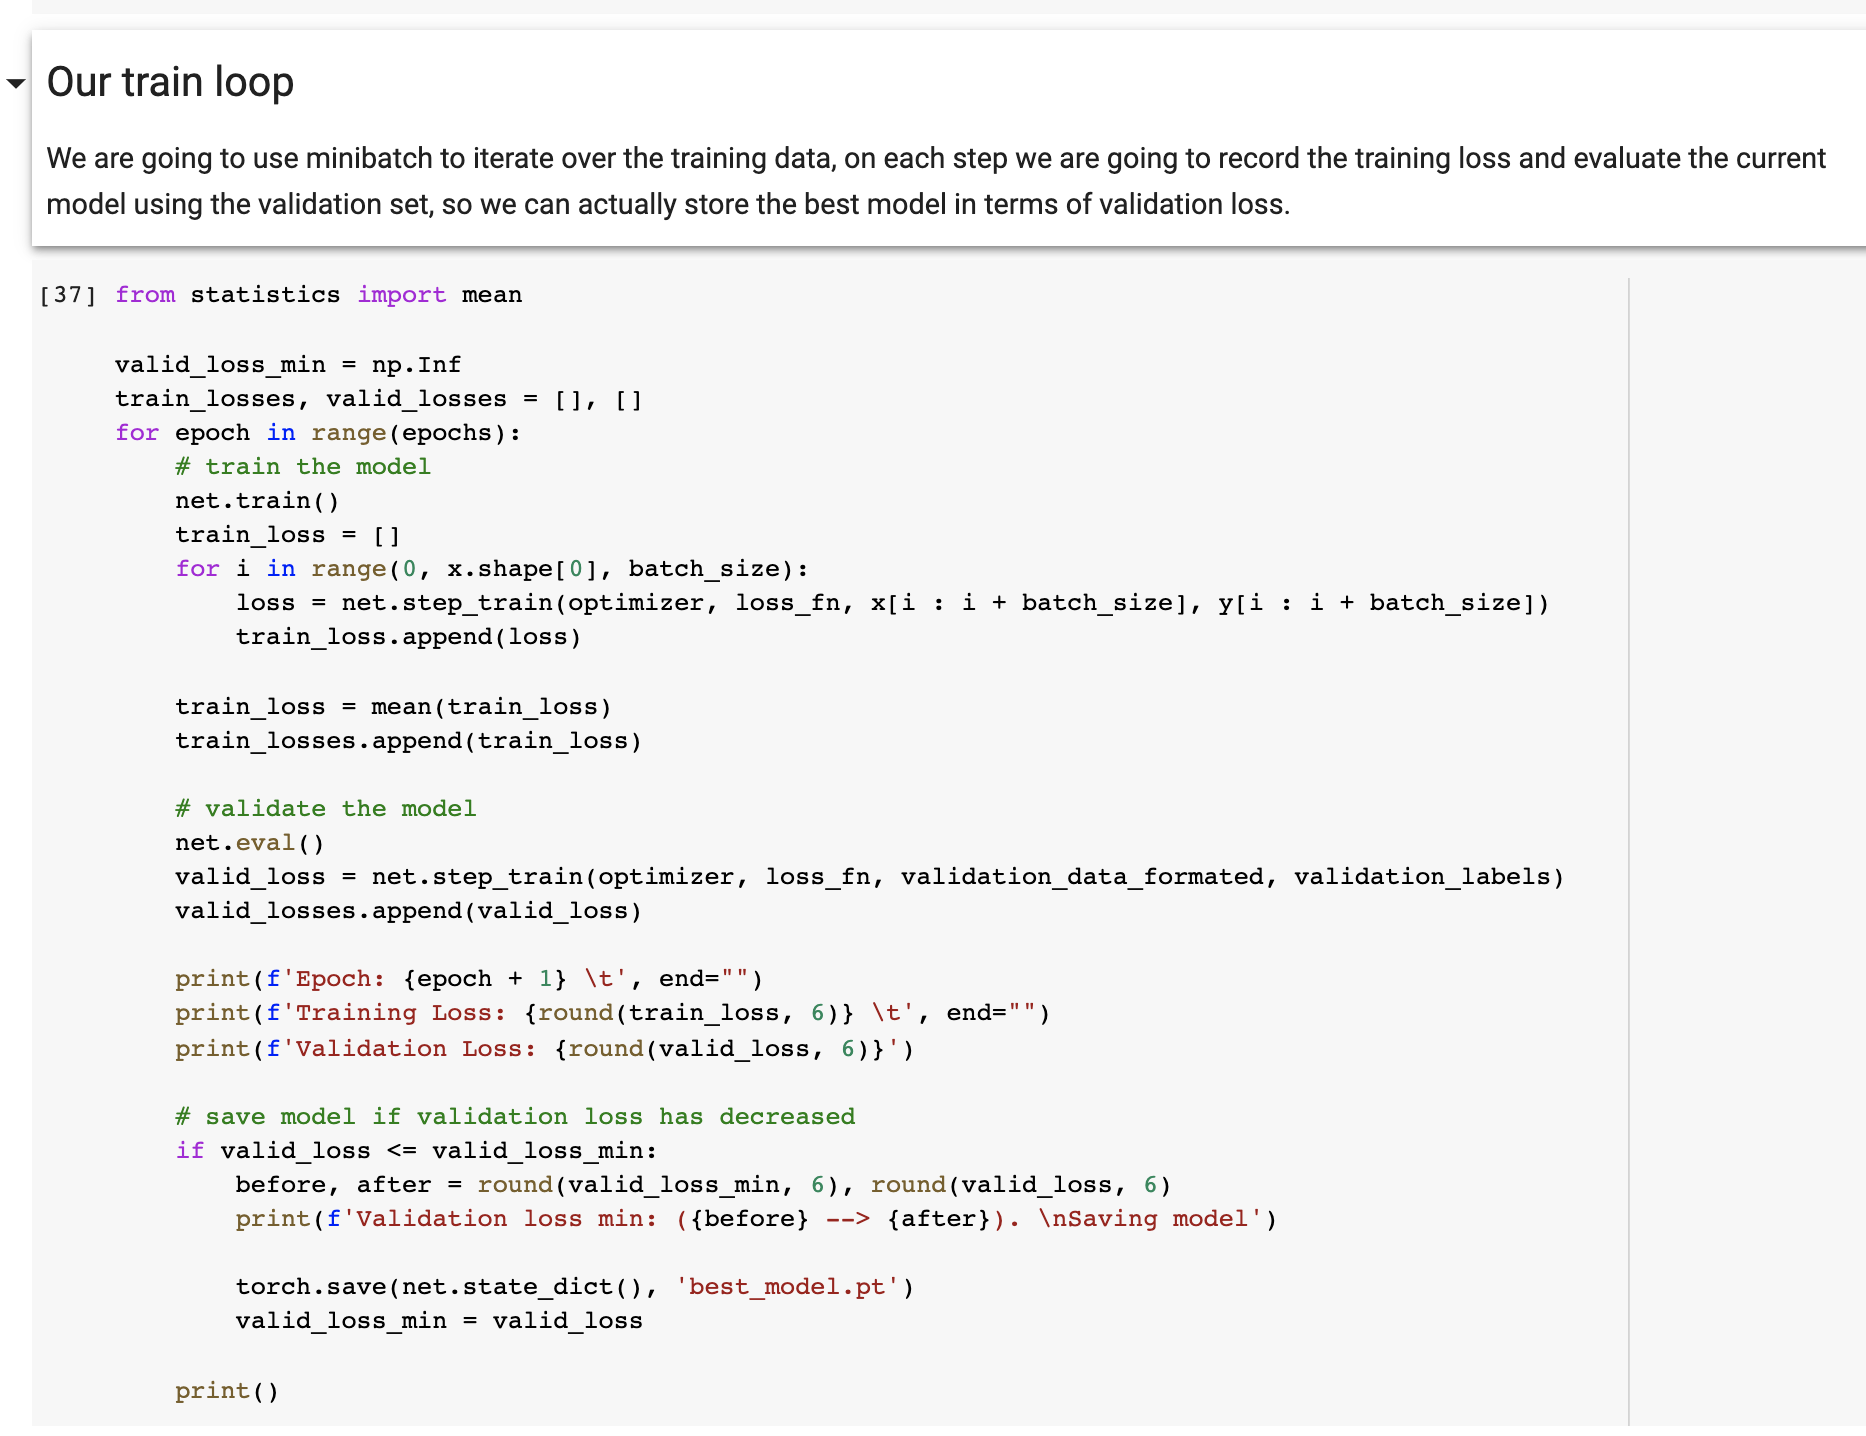
\includegraphics[width=0.85\textwidth]{9}
        \end{figure}

        \clearpage

        \section{Evaluación}

        Lo que hicimos para evaluar al sistema fue:
        \begin{itemize}
            \item Crear otro widget que nos permita explorar el dataset de prueba pero añadir la predicción del modelo
            en datos que nunca había visto para que podamos entender de manera intuitiva como va
            \item Creamos también una función auxiliar que toma todo el conjunto de test y nos regresa el accuracy
            para que podamos compararlo, que en mi caso me siento muy impresionado por el mismo.
        \end{itemize}

        \begin{figure}[h!]
            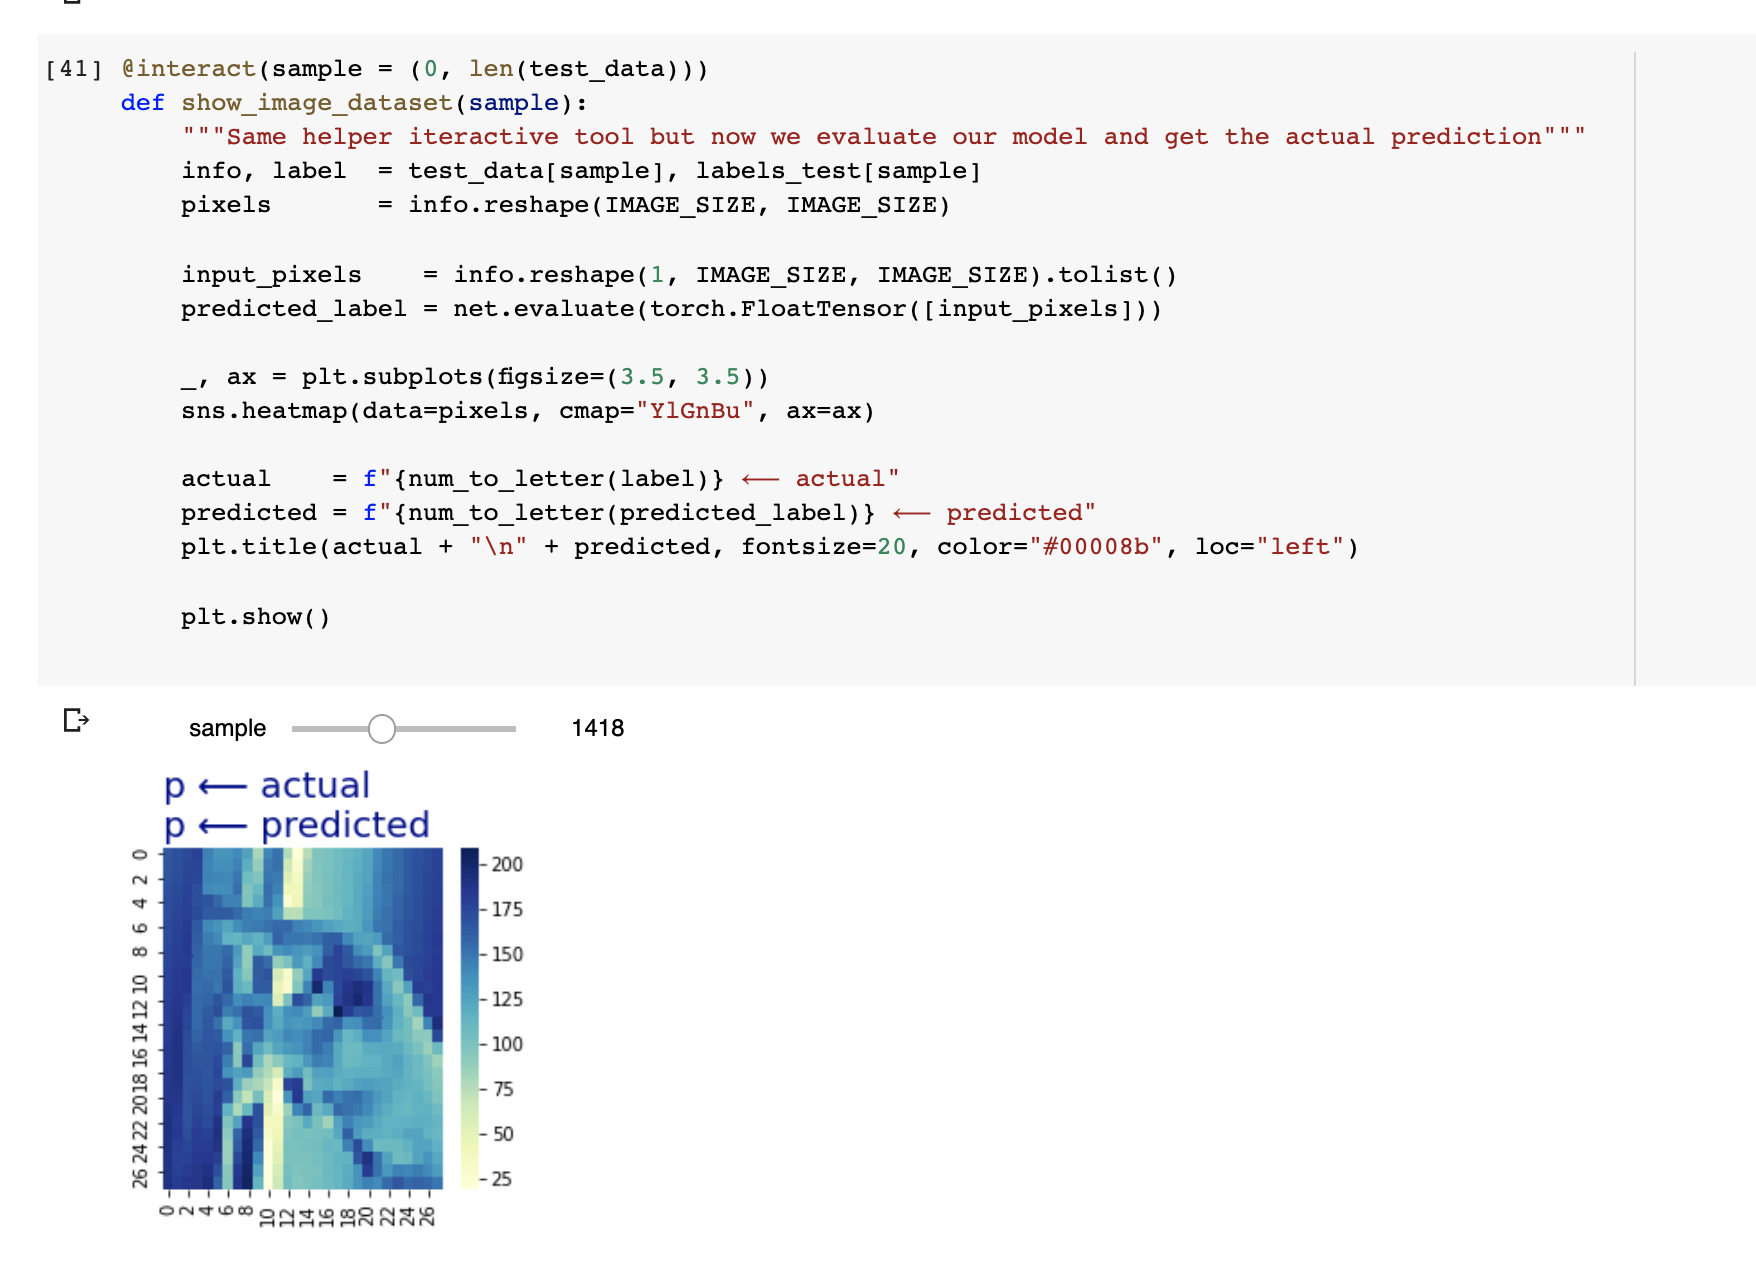
\includegraphics[width=0.45\textwidth]{10}
        \end{figure}

        \begin{figure}[h!]
            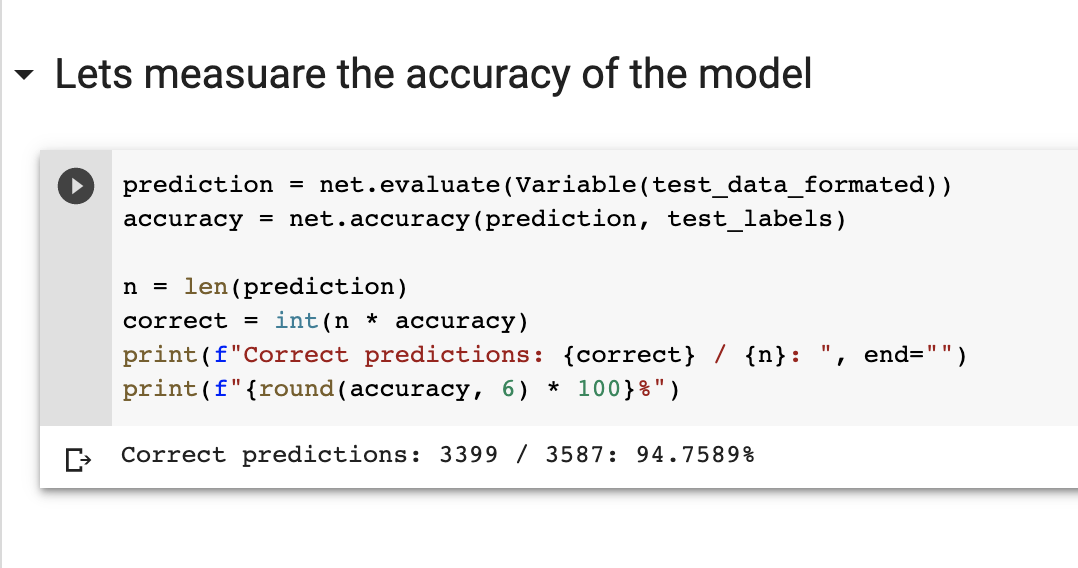
\includegraphics[width=0.45\textwidth]{11}
        \end{figure}

        En este podemos ver inmediatamente que nuestro sistema cumplio nuestro objetivo, 
        logran un mas de 85\% de accuracy en el conjunto de prueba.


        \subsection{Codigo}
        \subsubsection{Codigo principal}
        Se encuentra el Google Colab añado un pdf con la version mas actual pero recomiendo de gran medida correrlo por ustedes
        mismos haciendo click en el link:
        \url{https://colab.research.google.com/drive/1ms7-m-3skncTgqDRMo8lTeLjwZne4hAy#offline=true&sandboxMode=true}
        
        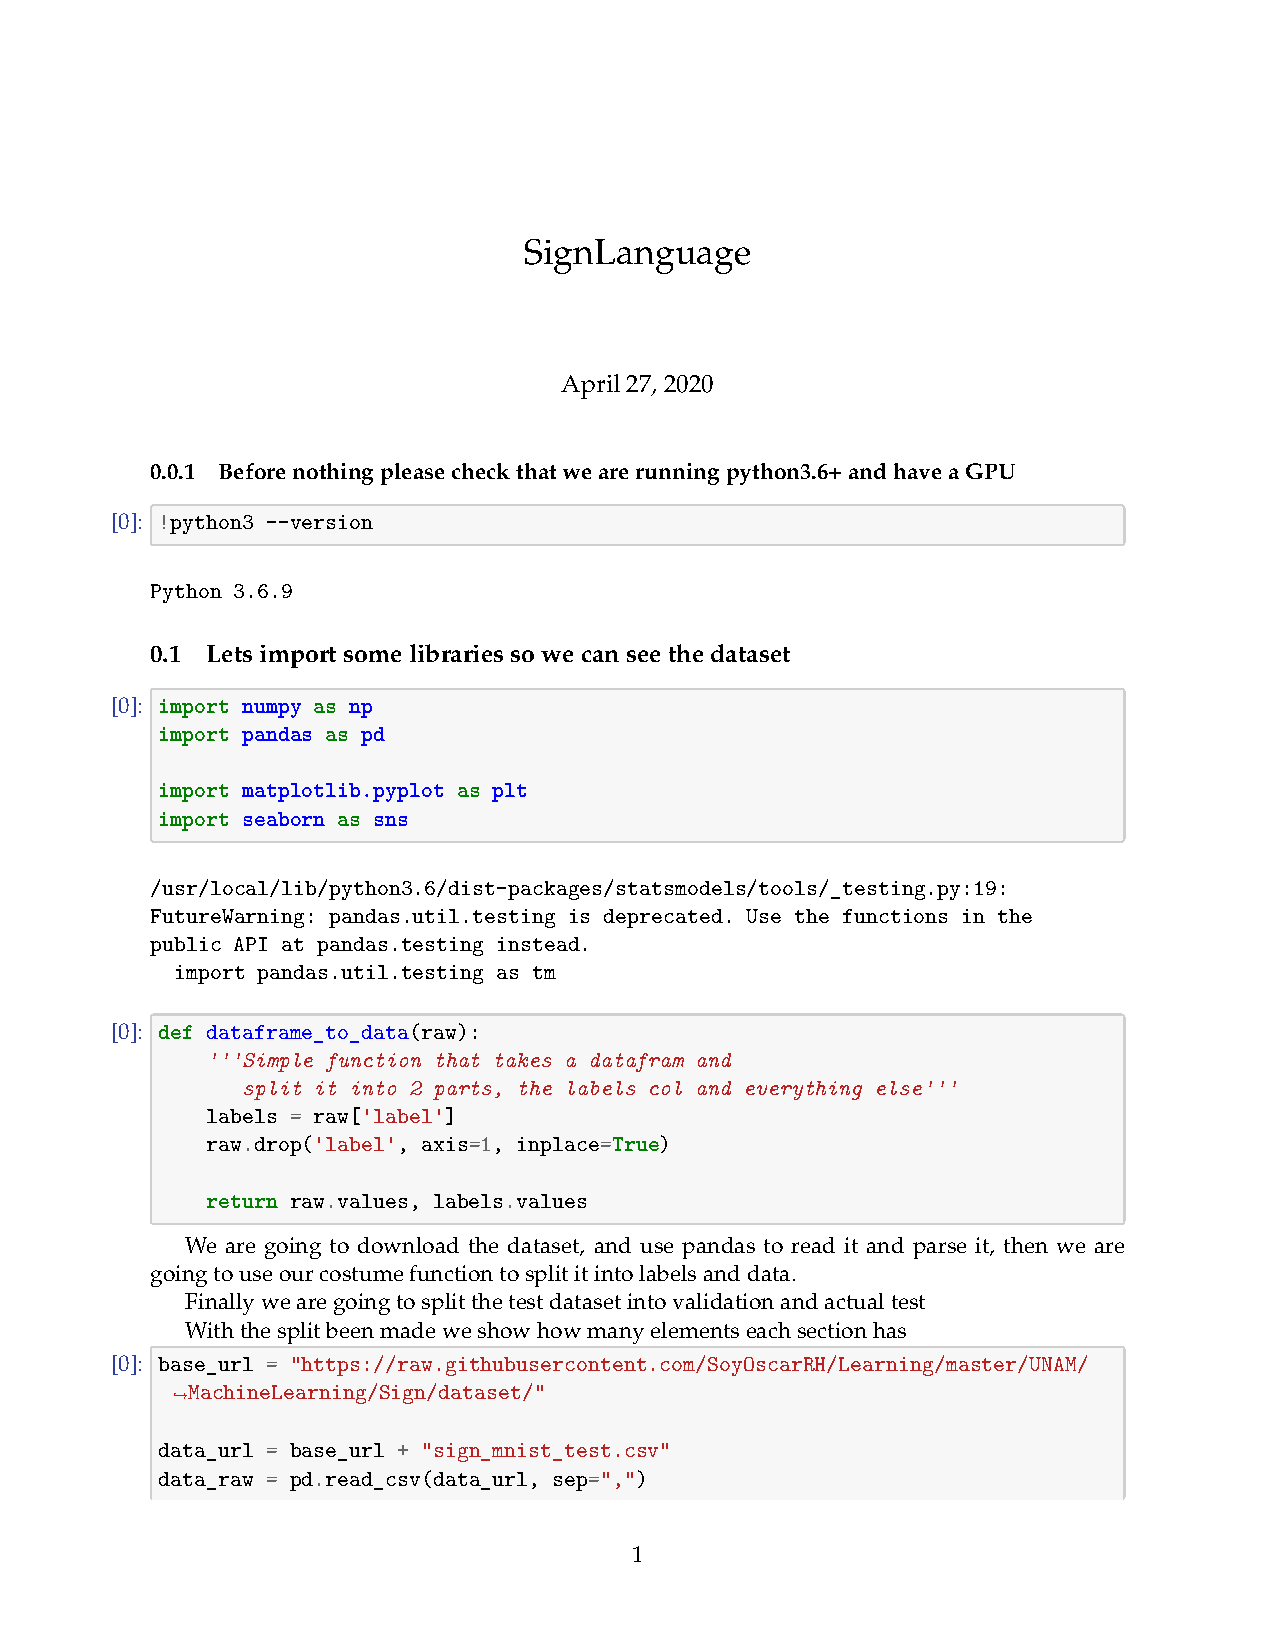
\includepdf[pages=-,pagecommand={},width=\textwidth]{Graphics/SignLanguage.pdf}

        \section{Experimentos}
            En general, esta idea para la implementación la base en implementaciones pasadas que había hecho para clasificar
            el dataset de CIFRA-10 a este le retire una capa convolucional y pase de un kernel de 5x5 a uno de 3x3 pensando en
            que con esta baja resolución y en blanco y negro no quería perder detalles importantes muy rápidamente,
            todo esto ayudo a mejorar notablemente el desempeño.
            
            El siguiente paso fue colocar potencias de dos de tal manera de que optimizara el cache de la mejor manera, es decir
            usando batch de 64 y teniendo 256 neuronas ocultas.
            Esto termino sin afectar de una manera significa el resultado.
            
            Finalmente y lo que si afecto en gran medida fue la cantidad de iteraciones que daba y el learning\_rate, al principio
            al entrenarla en mi laptop lo máximo que podía esperar eran 5 iteraciones pero bajando el learning rate y dando espacio
            a más iteraciones fue la clave para pasar el 83\% al 95\%. :D
            
            Otro experimento que intente era cambiar la probabilidad del dropout, pero tampoco obtuve mejoras significativas por lo
            que lo deje en el que daba el mejor resultado que es alrededor del 0.5.
        \section{Posibles mejoras a futuro}

            \begin{itemize}
                \item Podríamos usar menos capas profundas para poder estudiar de mejor manera los filtros resultantes, o en
                general creo que seria una buena idea usar mapas de activación para ver que están haciendo los filtros
                \item Probar este tipo de arquitectura en un dataset con más definición y al final con color de tan manera que
                podemos entender si el color de la piel juega un papel aquí
                \item Podríamos probar con pequeños gifs, es decir secuencias de fotogramas para poder representar las últimas dos
                letras faltantes. (seria interesante probar redes recurrente + convolucionales).
            \end{itemize}

        \section{Conclusión}

        Gracias a los resultados vimos que es posible crear un algoritmo con la ayuda de las redes neuronales
        que nos permite clasificar con un gran desempeño la letra dada una imagen de una mano realizando ese símbolo
        en lenguaje americano de señas.


\begin{thebibliography}{10}

  \bibitem{1} 
      \textit{Aidan Wilson}, 
      Sep 29, 2019 \\
      \url{https://towardsdatascience.com/a-brief-introduction-to-supervised-learning}

  \bibitem{Sand} 
      Apr 27, 2020 \\
      \url{https://stanford.edu/~shervine/teaching/cs-230/cheatsheet-convolutional-neural-networks}


\end{thebibliography}



\end{document}